\documentclass[12pt, a4paper]{article}

% Font
\usepackage[utf8]{inputenc}
\usepackage{MinionPro} 
\input{glyphtounicode}
\pdfgentounicode=1 
\usepackage{microtype}
\usepackage[super]{nth}

 % Format
\setlength{\parindent}{0.5in}
\setcounter{secnumdepth}{0}
\usepackage{authblk}
\renewcommand\Affilfont{\small}
\usepackage[hang, flushmargin]{footmisc}

% Language
\usepackage[british]{babel}

% Links
\usepackage[colorlinks = true, linkcolor = black, urlcolor = black, citecolor = black]{hyperref} 

% Figures
\usepackage{graphicx}
\usepackage[small, labelfont = bf, labelsep = newline]{caption}

% Tables
\usepackage{booktabs}
\usepackage{tabularx}
\usepackage[table, xcdraw]{xcolor}

% References
\usepackage{csquotes}
\usepackage[style = apa]{biblatex}
\addbibresource{references.bib}

% Frontmatter
\title{Intergroup contact fosters\\more inclusive social identities\thanks{Reimer, N. K., Kamble, S. V., Schmid, K., \& Hewstone, M. (in press). Intergroup contact fosters more inclusive social identities. \textit{Group Processes \& Intergroup Relations.}}}
\author[1]{Nils Karl Reimer}
\author[2]{Shanmukh V. Kamble}
\author[3]{Katharina Schmid}
\author[1]{Miles Hewstone}
\affil[1]{University of Oxford, United Kingdom}
\affil[2]{Karnatak University Dharwad, India}
\affil[3]{Universitat Ramon Llull, ESADE Business School, Spain}
\date{June 25, 2020}

\begin{document}

\maketitle

\begin{abstract}
\noindent We examined how people construct their social identities from multiple group memberships---and whether intergroup contact can reduce prejudice by fostering more inclusive social identities. South Indian participants ($N = 351$) from diverse caste backgrounds viewed 24 identity cards, each representing a person with whom participants shared none, one, two, or all of three group memberships (caste, religion, nationality). Participants judged each person as “us” or “not us”, showing whom they included in their ingroup, and whom they excluded. Participants tended to exclude caste and religious minorities, replicating persistent social divides. Bridging these divides, cross-group friendship was associated with more inclusive identities which, in turn, were associated with more positive relations between an advantaged, an intermediate, and a disadvantaged caste group. Negative contact was associated with less inclusive identities. Contact and identity processes, however, did not affect entrenched opposition to (or undermine support for) affirmative action in advantaged and disadvantaged groups.\\[1ex]
\noindent \textbf{Keywords:} intergroup contact, social identity, multiple categorization, interminority relations, perceived discrimination, affirmative action \\[1ex]
\end{abstract}

\noindent How we feel about and act toward others depends on whom we consider “us” and “them”---that is, whom we include in, and exclude from, our ingroup \parencite[for a review, see][]{reimer_self-categorization_2020}. In some situations, this distinction rests on one salient categorization, for example, someone’s nationality at an international border. In diverse societies, however, this distinction often depends on multiple, overlapping group memberships. Individuals differ in how they construct their ingroup from these group memberships. Some espouse narrow definitions of who is “us” and “them”, while others adopt more inclusive identities. Many Americans, for example, associate being American with being White \parencite{devos_american_2005}. This suggests that whom Americans consider “us” and “them” might depend on someone’s race \emph{and} nationality. In this paper, we examine how people construct their social identities from multiple group memberships---and whether intergroup contact can reduce prejudice by fostering more inclusive social identities. We use a novel method to study social identification across multiple social categories and to examine possible antecedents (intergroup contact, social dominance orientation) and consequences (intergroup attitudes, support for affirmative action, intergroup threat) of more inclusive identities.

Social psychologists have highlighted the importance of considering two \parencite{berry_immigration_1997, crisp_multiple_2007, dovidio_commonality_2009} or more \parencite{roccas_social_2002} social categories for understanding intergroup relations. \textcite{crisp_multiple_2007} reviewed evidence that we tend to have more favourable attitudes towards people with whom we share some, but not all, group memberships than towards people with whom we do not share any group memberships. \textcite{gaertner_reducing_2000} showed that espousing a more inclusive common ingroup identity (e.g., Indian) over a narrower identity (e.g., Hindu) can extend the benefits of ingroup favouritism to outgroup members and thus reduce intergroup bias. \textcite{roccas_social_2002} recognized that, though we all hold multiple overlapping group memberships, we differ in how we construct our social identities from them. Broadly, these perspectives recognize that we belong to multiple overlapping groups; that we use these group memberships to construct a subjective sense of who is “us” and “them”; and that espousing more inclusive social identities can reduce prejudice and discrimination.

Diverse societies confront their members with the decision of which intersections of various group memberships to include in their ingroup. One Indian Hindu, for example, might restrict their ingroup to people of the same nationality, religion, and caste. Another Indian Hindu might consider all Indians, whatever their caste or religion, as ingroup members (Figure~\ref{fig:f1}). Past research \parencite{van_dommelen_construing_2015} indeed observed substantial individual differences in whom participants considered “us” and “not us”. Some participants espoused more inclusive social identities---that is, they included more people in their subjective ingroup. Other participants espoused less inclusive social identities---that is, they included fewer people in their subjective ingroup. All participants \parencite[studied by][]{van_dommelen_construing_2015}, however, belonged to the same disadvantaged minority group. Past research thus provided evidence for individual differences, but did not examine group differences in whom people consider “us” and “not us”.

\begin{figure}
\centering
\caption{
Schematic representations of social identity structures \protect\parencite{roccas_social_2002}, ordered by their social identity inclusiveness \protect\parencite{van_dommelen_construing_2015}
}
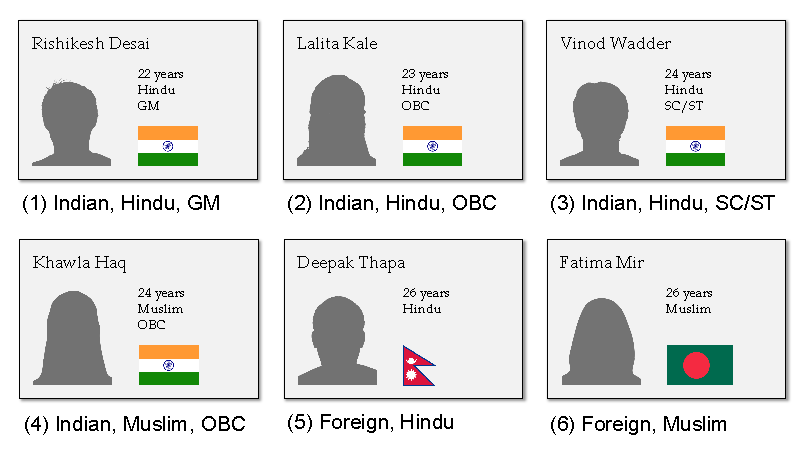
\includegraphics[scale=1]{../figures/figure-1}
\caption*{\textit{Note.} Shaded regions represent the groups which a participant has to categorize as “us” to be assigned that structure. An Indian Hindu, for example, might consider only people who share their nationality, religion, and caste as ingroup members (\emph{intersection}). Someone else might consider all their fellow Indians, whatever their religion or caste, as ingroup members (\emph{dominance}). Another person might consider anyone who shares their nationality or religion as ingroup members (\emph{merger}).}
\label{fig:f1}
\end{figure}

Group membership, however, often shapes whom people include in, and exclude from, their subjective ingroup. For majority-group members, negotiating their ethnic and national identities means something different than for minority-group members \parencite[for a review, see][]{dovidio_commonality_2009}. Majority-group members face the choice of including or excluding ethnic, religious, and other minorities from their subjective ingroup. Choosing to include or exclude minorities could, for example, reflect whether a majority-group member holds multicultural or nativist views. Minority-group members face the choice of aligning themselves with the dominant majority group or seeking a common ingroup identity with other minority groups. We expect that group differences are as great as, if not greater than, individual differences in social identity construals---especially if groups differ in status and power. Our research includes participants from advantaged, intermediate, and disadvantaged backgrounds to study how groups differ in terms of whom their members consider “us” and “not us”.

How we think and feel about others depends on whether we include them in our ingroup. Dividing others into “us” and “not us” is thus a necessary and sufficient condition for ingroup favouritism \parencite{tajfel_human_1981}. Past research has shown that people favour ingroup members in resource allocation \parencite{tajfel_social_1971}, in causal attribution \parencite{hewstone_ultimate_1990, taylor_ethnocentrism_1974}, in helping behaviour \parencite{levine_identity_2005}, in information processing \parencite{van_bavel_neural_2008}, and in evaluation \parencite{otten_evidence_2000}. Considering more people as “us” should extend ingroup favouritism to a wider range of people, and thus reduce prejudice and discrimination \parencite[for a review, see][]{nelson_common_2016}. Our research examines whether fostering more inclusive social identities leads to more favourable attitudes and less social distance toward national, religious, and caste outgroups.

Contact with members of other groups changes how we think and feel about them. Past research has shown that intergroup contact reduces prejudice \parencite{pettigrew_meta-analytic_2006} by decreasing intergroup anxiety, increasing empathy and perspective-taking, and by increasing knowledge about the other group \parencite{pettigrew_how_2008}. In addition, researchers have proposed that contact could reduce prejudice by changing how we see ourselves \parencite{pettigrew_generalized_1997, pettigrew_intergroup_1998}. Encountering diverse others could initiate a process of cognitive differentiation \parencite{kramer_social_2011} whereby individuals become aware of complex interrelations between their group memberships and adopt more complex social identities \parencite{schmid_antecedents_2009}---that is, they become aware that they belong to multiple categories and recognize that these multiple categories do not always overlap \parencite{van_dommelen_construing_2015}. Other research has found that intergroup contact can, under the right conditions, motivate people to adopt a more inclusive common ingroup identity \parencite{gaertner_contact_1994} and to include the outgroup in their self-concept \parencite{page-gould_understanding_2010}. If intergroup contact motivates people to adopt social identities that include outgroup members, it should reduce prejudice and discrimination against them. Our research examines whether intergroup contact can reduce prejudice against religious and caste outgroups by fostering social identities that include them as ingroup members.

Beyond prejudice, researchers have debated whether, by fostering more inclusive identities, intergroup contact helps or hinders social change. Social change often requires advantaged and disadvantaged groups to strive for redistributive policies. On the one hand, fostering inclusive identities could break down the boundaries between the advantaged ingroup and the disadvantaged outgroup---turning injustice faced by “them” into “our” problem. This process could narrow the gap between advantaged-group members’ support for the principle of equality and their opposition to its implementation \parencite{dixon_intergroup_2007}. On the other hand, fostering more inclusive identities could distract disadvantaged-group members from differences in resources and power, and thus reduce their demands for and support for social change \parencite{dixon_attitudes_2012, saguy_irony_2009}. Together, these mechanisms suggest that fostering more inclusive identities could increase support for social change among the advantaged, but decrease support among the disadvantaged. Our research examines how intergroup contact, by fostering more inclusive social identities, affects support for affirmative action policies, as well as perceptions of relative (dis-)advantage, in advantaged and disadvantaged groups.

Most research on intergroup relations examines relations between an advantaged majority group and a disadvantaged minority group. Most social contexts, however, feature various groups facing various disadvantages. \textcite{craig_coalition_2012} argued that racial minorities may respond to the disadvantages they face by derogating other racial minorities or by forming a coalition with them. They showed that perceiving discrimination can, as far as it fosters a shared ingroup identity with other disadvantaged groups, improve interminority relations. \textcite{vollhardt_inclusive_2016} observed that South Indians from disadvantaged caste and religious groups were more likely to express support for another disadvantaged group when they recognized similarities between their own and other groups’ experiences of discrimination. \textcite{dixon_contact_2017} found that Indian Muslims who reported having more contact with other disadvantaged groups were also more likely to recognize shared grievances and to express support for collective action benefiting all disadvantaged groups. Our research adds to this literature by examining intergroup relations between two disadvantaged groups, one of which occupies an intermediate position in the social hierarchy. We examine whether, by fostering shared ingroup identities, contact between disadvantaged groups can foster more positive intergroup relations, shared perceptions of disadvantage, and mutual support for affirmative action.

\subsection{Caste, Religion, Nation in South India}

We investigated these questions in the context of caste, religion, and nationality in South India. India provides an important context for studying social identification across multiple social categories. India is diverse. Indians belong to different castes, religions, and other groups that intersect in numerous ways. India is also underrepresented in psychological research.\footnote{Among the societies underrepresented in psychological research (Henrich et al., 2010), India is a prominent omission as it spans almost a fifth of the world’s population.} Few studies of intergroup relations \parencite[e.g.,][]{ghosh_hindu-muslim_1991, tausch_relationships_2009} focus on religious relations in India. Even fewer \parencite[e.g.,][]{cotterill_ideological_2014} focus on caste relations. Our research examined the cross-cutting categories of caste, religion, and nationality in a diverse sample of South Indian students.

Caste is a system of social relations that concentrates resources in the hands of dominant castes by restricting subordinate castes’ occupations and by enforcing segregation and endogamy \parencite{jodhka_caste_2012}. This system is underpinned by a tradition that conveys caste through markers such as surname and diet, ranks castes according to their supposed ritual purity, and condemns contact with supposedly less pure castes. This tradition includes the practice of untouchability which excludes some castes from public life and consigns them to landlessness and menial labour. Dalits, members of castes that have been subjected to untouchability, still face interpersonal discrimination and economic inequalities resulting from this (now illegal) practice. Since Independence, the Indian State has sought to redress caste-based injustices by reserving seats in state-run universities and state-sector jobs for ‘Scheduled Castes’ (the official term for Dalits) and ‘Scheduled Tribes’ (the official term for Adivasi, India’s indigenous peoples). Reservation policies, along with persistent discrimination, mean that caste identities continue to structure people’s lives.

Caste identities have different meanings for disadvantaged, advantaged, and intermediate groups. For the most disadvantaged, caste is often defined by their experience of discrimination and their resistance against it \parencite{jodhka_caste_2012}. Dalits have built movements to assert their economic and political rights---founding, for example, the Bahujan Samaj Party in 1984---and thus created a positive identity around their resistance against oppression. Dalits, however, often face violent backlash when asserting their rights \parencite[e.g.,][]{noauthor_15_2017}. For the most advantaged, Dalit emancipation threatens their social and economic dominance. Reservation policies, for example, restrict access to university seats for upper-caste applicants who must compete with all other applicants in the ‘General Merit’ category. Other groups occupy an intermediate position in the caste hierarchy. In 1990, the government extended reservations to ‘Other Backward Classes’, that is, communities that were socially and educationally disadvantaged, but had not been subjected to untouchability. For intermediate groups, caste is often defined by the question whether they can gain or maintain access to reserved university seats and government jobs. As a result, caste identities remain important in Indian politics.

South India is religiously diverse. In Karnataka, where we conducted this research, 84\% of inhabitants are Hindus, while 13\% are Muslims. Muslims face both structural inequalities and communal violence. In 2002, for example, over a thousand Muslims were killed in a pogrom in Gujarat \parencite{dhattiwala_political_2012}. In recent years, anti-Muslim violence has been increasing \parencite{amnesty_international_india:_2017}. Religion is intertwined with two currents of Indian nationalism \parencite{katz_hindu_2009}. On the one hand, the secular foundations of the Indian State resulted from an inclusive nationalism that strives to include Indians of all religions. On the other hand, Hindu nationalism (Hindutva) is an ideology that equates being Indian with being Hindu, thus excluding Muslims from the national identity. Narendra Modi’s Bharatiya Janata Party (BJP) government espouses Hindutva and enjoyed broad support at the time of our study \parencite{pew_research_center_three_2017}. Indians thus face a choice between two ideologies that either include Indian Muslims in the national identity or exclude them from it.

\subsection{Present research}

Our research used a novel method to study social identification across multiple categories in a sample of South Indians from diverse caste backgrounds. We examined how people construct their social identities from multiple group memberships, whether intergroup contact is associated with more inclusive social identities, and how more inclusive social identities relate to prejudice and support for social change. Below, we introduce the experimental task before reviewing our research questions and hypotheses.

We adapted the triple crossed-categorization task \parencite{van_dommelen_construing_2015} to assess how participants construct their social identities from multiple group memberships. In this task, participants view identity cards, each representing a person with whom participants shared none, one, two, or all of three group memberships. Participants report whether they consider each person as “us” or “not us”, showing whom they include in, or exclude from, their ingroup. This task allowed us to study identification across multiple social categories and how it relates to the predictors and outcomes in our hypotheses. Van Dommelen et al. \citeyear{van_dommelen_construing_2015} used a similar task to examine whom participants considered “us” and “not us”. However, their research included participants from only one group, aggregated participants’ categorizations into a single score, and tested whether that score correlated with aggregated responses to contact and attitude measures. Our research included participants from multiple groups and used multilevel modeling to test whether contact with and attitudes toward \emph{each} group were associated with the inclusion of \emph{that} group in one’s social identity. This allowed for a more fine-grained analysis of individual and group differences in identification across multiple social categories.

We pursued four research questions. First, we examined how participants’ group memberships shaped whom they included in, and excluded from, their ingroup (\emph{group differences}). We hypothesized that participants would exclude targets from religious and national outgroups---and that participants from advantaged castes would exclude targets from disadvantaged castes, and vice versa. We did not have a clear prediction for participants from intermediate backgrounds. Second, we examined whether past experiences with members of caste and religious outgroups shaped whom participants included in, and excluded from, their ingroup (\emph{individual differences}). We hypothesized that positive contact and cross-group friendship would be associated with more---and negative contact \parencite{barlow_contact_2012, hayward_toward_2017} with less---inclusive social identities. Third, we examined whether, by fostering more inclusive social identities, intergroup contact would be associated with less prejudice (\emph{intergroup attitudes}). We hypothesized that categorizing someone as “us” would be associated with more favourable attitudes and less social distance toward that person. Fourth, we examined how intergroup contact, by fostering more inclusive social identities, affects support for affirmative action in advantaged and disadvantaged groups (\emph{support for social change}). We hypothesized that more inclusive social identities would be associated with less perceived discrimination and less support for affirmative action among the disadvantaged, and with more perceived privilege and more support for affirmative action among the advantaged.

In addition, we explored how two other constructs related to more inclusive social identities. First, we examined ideological preferences for group dominance \parencite{sidanius_social_1999} as an additional predictor variable to rule out a potential confound, whereby people high in social dominance orientation might both eschew contact with caste and religious minorities and exclude them from the common ingroup. Second, we examined perceptions of intergroup threat as an additional outcome variable to test whether more inclusive identities were associated with this more distal outcome. Perceptions of intergroup threat play an important role in shaping intergroup relations \parencite[for a review, see][]{nelson_intergroup_2016}. We examined whether participants who included caste and religious minorities in their ingroup would, in addition to feeling more warmth and less social distance toward them, feel less threatened by them in terms of both realistic and symbolic threat. As we had not planned our study with clear directional predictions concerning social dominance orientation and intergroup threat, we consider these additional analyses exploratory.

\section{Method}

All materials, data, analysis scripts, and appendices are available online.\footnote{\protect\href{https://doi.org/10.17605/OSF.IO/QPCRM}{https://doi.org/10.17605/OSF.IO/QPCRM}} Here, we only report measures testing our hypotheses, omitting measures replicating earlier research or validating the experimental task (Appendix A). Reanalysing existing data \parencite{van_dommelen_construing_2015}, we determined that $\sim 100$ respondents per group would allow reasonably precise estimates of model parameters (Appendix B). We report descriptive statistics and correlations in Appendix C.

\subsection{Participants}

We recruited 351 students at Karnatak University (Dharwad, India). Of these, we excluded 49 participants who did not belong to any of four caste groups (n = 20), failed to indicate their caste group ($n = 7$), and/or reported Islam as their own or their family’s religion ($n = 27$).\footnote{Because Muslims---unlike Jains and Christians---featured in the experimental task, we would have had to consider them as a distinct group in the analyses. As this subsample was too small for any meaningful analyses, we instead opted to exclude Muslim participants.} This left 302 participants who reported Hinduism ($n = 286$), Jainism ($n = 8$), or Christianity ($n = 8$) as their or their family’s religion, and General Caste ($n = 99$), Other Backward Class ($n = 127$), Scheduled Caste ($n = 54$), or Scheduled Tribe ($n = 22$) as their caste group. Table~\ref{tab:t1} summarizes participants by gender, age, nationality, religion, and caste.

\begin{table}    
\caption{Participants by gender, age, nationality, religion, and caste. Categories in \textit{italics} were excluded from the final sample. N/A marks missing responses.}
\centering
\figureversion{lining, tabular}
\small	
\begin{tabular}{llrr} \addlinespace \toprule
\multicolumn{2}{l}{Category} & $n$ & \% \\ \midrule \addlinespace 
Gender      & Woman      & 215 & 61 \\
            & Man & 121 & 34 \\
            & Other & 0 & 0 \\
            & N/A & 15 & 4 \\ \addlinespace \addlinespace
Age         & 18--20 & 1 & 0 \\
            & 21--23 & 254 & 72 \\
            & 24--26 &  77 & 22 \\
            & 27--29 &  10 &  3 \\
            & 30--32 &   1 &  0 \\
            & 33--35 &   0 &  0 \\
            & 36 or older & 1 & 0 \\ 
            & N/A & 7 & 2 \\ \addlinespace \addlinespace
Nationality & Indian & 339 & 97 \\
            & Other & 0 & 0 \\
            & N/A & 12 & 3 \\ \addlinespace \addlinespace
Religion    & Buddhism & 1 & 0 \\ 
            & Christianity & 11 & 3 \\ 
            & Hinduism & 297 & 85 \\ 
            & \textit{Islam} & \textit{27} & \textit{8} \\ 
            & Jainism & 8 & 2 \\ 
            & Other & 2 & 1 \\ 
            & N/A & 5 & 1 \\ \addlinespace \addlinespace
Caste       & General Caste & 104 & 30 \\ 
            & Other Backward Class & 143 & 41 \\ 
            & Scheduled Caste & 54 & 15 \\ 
            & Scheduled Tribe & 23 & 7 \\ 
            & \textit{Other / Not applicable} & \textit{20} & \textit{6} \\ 
            & \textit{N/A} & \textit{7} & \textit{2} \\ \addlinespace \midrule
Total       &   & 351 & 100 \\ \bottomrule
\end{tabular}
\label{tab:t1}
\end{table}

\subsection{Procedure}

Participants completed a triple crossed-categorization task, in which they viewed 24 identity cards. Each showed a fictitious person’s name, age, religion, nationality, caste reservation, and a head-and-shoulders silhouette. Based on a pilot study, we manipulated the target’s caste, religion, and nationality such that each target represented a person with whom participants shared none, one, two, or three group memberships (Figure~\ref{fig:f2}). We tested participants in classrooms of 24--71 students by presenting targets in a slide-based presentation and by handing each student a pen-and-paper questionnaire. Each slide contained a male and a female target with participants focusing on the target corresponding to their gender. Slides also contained a number identifying each target, and response scale(s) corresponding to the question(s) participants answered at the time.

\begin{figure}
\caption{Examples of targets used in the triple crossed-categorization task}
\centering
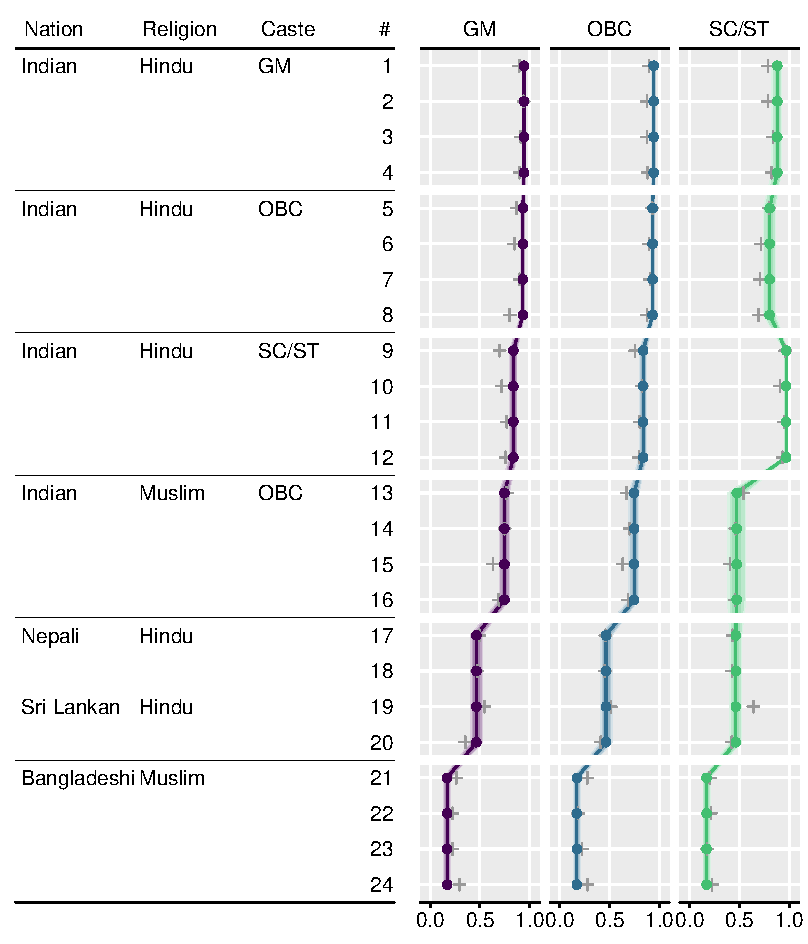
\includegraphics[scale=1]{../figures/figure-2}
\caption*{\textit{Note.} Based on ratings in a pilot study ($N = 26$), we selected the four most prototypical targets (out of fifty initial targets) for each of six plausible combinations of caste, religion, and nationality (for details, see Appendix~D). Each target showed a person's caste reservation (GM = General Merit, OBC = Other Backward Class, SC/ST = Scheduled Caste/Scheduled Tribe), religion (Hindu, Muslim), and nationality (Indian, Nepali, Sri Lankan, Bangladeshi). Each target also showed the person's first and last name, age (21--26 years), and a silhouette corresponding to the person's gender \protect\parencite[adapted from][]{ma_chicago_2015}. Each target's age and silhouette, as well as the order in which the targets were presented, varied across sessions.}
\label{fig:f2}
\end{figure}

In each session, participants first familiarized themselves with each target (shown for 7 s in a randomized order) in an automated slide show. Participants viewed targets (in the same order) for a second time, noting for each target whether they felt that this person was one of their own group (1 = “us”), or not one of their own group (0 = “not us”). Participants viewed targets for a third time, rating how comfortable or uncomfortable they would feel to share a room with this person (social distance; 1 = \textit{very uncomfortable}, 7 = \textit{very comfortable}), and how they felt toward this person (feeling thermometer; 0 = \textit{cold}, 100 = \textit{warm}). Participants then completed the measures described below.

\subsection{Measures}

We report one of two reliability indices for our measures, the Spearman-Brown statistic ($\rho$) for two-item measures \parencite{eisinga_reliability_2013} and McDonald’s omega ($\omega$) for multi-item measures \parencite{dunn_alpha_2014}.

We measured intergroup contact as: how often, from 1 = \textit{never} to 5 = \textit{very often,} participants meet outgroup members in their everyday life (contact quantity), and how often, on average, they have positive/good contact and negative/bad contact with outgroup members \parencite{barlow_contact_2012}. We preceded these items with examples of positive and negative contact experiences. We measured cross-group friendship with two items \parencite{turner_reducing_2007}: “How many close friends do you have who are [outgroup members]?” (1 = \textit{none}, 5 = \textit{more than ten}), and “How often do you spend time with [outgroup] friends?” (1 = \textit{never} to 5 = \textit{very often}; $.65 < \rho < .71$). Participants reported contact with four groups: Dalits, people from other backward classes, people from general castes, and Muslims.

We measured social dominance orientation as how much, between 1 = \textit{strongly oppose }and 7 = \textit{strongly favour}, participants endorsed eight statements about social hierarchies \parencite{ho_nature_2015}. Four items measured support for group-based dominance (SDO-Dominance), for example, “some groups of people are simply inferior to other groups”. Four items measured opposition to egalitarian ideologies (SDO-Egalitarianism), for example, “it is unjust to try to make groups equal”.\footnote{Replicating \protect\textcite['s][]{ho_nature_2015} findings, we found a four-factor model (with two method factors) to represent the data better than the one-factor ($\Delta\chi^2 = 155.14, p < .001$) or two-factor ($\Delta\chi^2 = 138.67, p < .001$) alternatives. Accounting for this structure, we used latent factor scores for SDO-Dominance and SDO-Egalitarianism in our analyses.}

We measured realistic threat---from Muslims and Dalits---with three items per outgroup \parencite{schmid_reducing_2014}, e.g., “the more power [Muslims/Dalits] gain in this country, the more difficult it is for [Hindus/people from my caste group]” (1 = \textit{strongly disagree}, 5 = \textit{strongly agree}; $\omega_\textit{Muslims} = .71, \omega_\textit{Dalits} = .79$). Two items measured symbolic threat, e.g., “[Muslims/Dalits] threaten [Hindus’/my caste group’s] way of life” (1 = \textit{strongly disagree}, 5 = \textit{strongly agree}; $\rho_\textit{Muslims} = .61, \rho_\textit{Dalits} = .65$).

We measured perceived (dis-)advantage as how easy or hard participants thought it was, on average, for people from various groups to succeed in India today (1 = \textit{very hard}, 7 = \textit{very easy}). Participants rated seven groups: People from your own background, Scheduled Caste, Scheduled Tribe, Other Backward Class, General Caste, Hindus, and Muslims.

Five items measured policy support. Participants read that “currently, 22.5\% of seats in central-government funded universities are reserved for Scheduled Caste and Scheduled Tribe students”, and that “an additional 27.5\% of seats in central-government funded universities are reserved for students from Other Backward Classes”. Participants indicated to what extent they opposed or supported reservation in higher education for students from each group (1 = \textit{strongly oppose}, 5 = \textit{strongly support}), and whether they thought that reservation in higher education for students from that group should increase, decrease, or remain unchanged (1 = \textit{decrease a lot}, 5 = \textit{increase a lot}; $\rho_\text{SC/ST} = .80, \rho_\text{OBC} = .80$). Participants then read that “no seats in central-government funded universities are reserved for Muslim students nationally, though some states have introduced quotas for Muslim students”. Participants indicated to what extent they opposed or supported reservation for Muslim students.

\subsection{Analysis strategy}

To answer our research questions, we used various (generalized) linear regression models. Specifically, we examined: (1) \emph{group} and \emph{individual differences} in how likely participants were to categorize different targets as “us” in a series of multilevel logistic models with participants’ target categorizations (1 = “us”, 0 = “not us”) as outcome variable; (2) consequences of participants’ target categorizations for \emph{intergroup attitudes} in a series of multilevel multivariate linear models with participants’ target-wise social distance and feeling thermometer ratings as outcome variables; and (3) consequences for \emph{support for social change} in a series of multivariate linear models with participants’ group-wise perceived (dis-)advantage and policy support ratings as outcome variables. We also explored whether participants’ target categorizations were associated with their intergroup threat ratings using multilevel linear models.

We estimated models in RStan \parencite{stan_development_team_rstan:_2020} using Bayes\-ian statistical methods. Bayesian inference involves choosing a likelihood function and prior distributions. The likelihood function links the observed data to one or more model parameters (e.g., regression coefficients) and states how likely the observed data are given different values of said model parameters. Our models derived the likelihood of the observed responses from a generalized linear model with a logit link function or a linear model with a (multivariate) normal distribution. Prior distributions state how plausible different values of said model parameters are before considering the observed data. Our models assigned conservative, weakly informative prior distributions to all model parameters \parencite{gelman_prior_2017}.\footnote{Specifically, we used $\beta \sim \text{Student-t}(2.5, 0, 1)$ for fixed effects in logistic models, $\beta \sim \text{Normal}(0, 1)$ for fixed effects in linear models, $\Omega \sim \text{LKJ}(4)$ for residual covariances in multivariate models, and $\sigma \sim \text{Half-Cauchy}(0, 1)$ for standard deviations of varying effects in multilevel models and for residual standard deviations in linear models.} Bayesian inference applies Bayes’ theorem to update prior distributions in light of the observed data to produce posterior distributions.\footnote{For a detailed introduction, consult \textcite{gelman_bayesian_2014}, \textcite{lambert_students_2018}, and \textcite{mcelreath_statistical_2016}.} Other than \textit{p}-values and confidence intervals, the resulting posterior distributions have a straight-forward interpretation as stating how plausible different values of the model parameters are given the observed data.

We tested our hypotheses in two steps. First, we compared models that corresponded to our hypotheses and selected the model that made the most accurate predictions. For example, we compared a model which estimated the probability of participants’ categorizing a target as “us” in the experimental task as \emph{varying} across the participants’ group memberships to a simpler model which constrained this probability to be \emph{fixed} across the participants’ group memberships. When the former made more accurate predictions than the latter, we considered this evidence that, as hypothesized, participants from advantaged and disadvantaged groups differed in how likely they were to categorize targets as “us”. Second, we inspected estimates from the selected model to examine whether model estimates were in the hypothesized direction. For example, we found that, as hypothesized, the selected model estimated advantaged-group participants to be less likely than disadvantaged-group participants to categorize disadvantaged-group targets as “us” ($\Pr = .80, [.73, .85]$ versus $\Pr =  .97, [.95, .98]$; $\Delta\Pr =  -.17, [-.23, -.12]$). For each model estimate, we report a point estimate and an uncertainty interval enclosing the 97\% most plausible estimates.

One way to compare statistical models is to estimate how well each model predicts observations \emph{within} the sample. This approach underlies comparison methods based on the relative log-likelihood of each model, such as likelihood-ratio tests or Bayes factors. This approach has well-known shortcomings, such as being sensitive to the specific prior distributions \parencite{gelman_bayesian_2014} and prone to overfitting \parencite{yarkoni_choosing_2017}. Instead, we compared models by estimating how well each predicts observations \emph{outside} the sample used to estimate it. We used 10-fold cross-validation, dividing observations into 10 folds, estimating model parameters using observations from 9 folds, calculating the model’s out-of-sample prediction accuracy for the remaining observations, and repeating the last two steps until we had estimated the model’s out-of-sample prediction accuracy for all observations.\footnote{Specifically, we used \emph{stratified} cross-validation to account for the nestedness of our observations, ensuring that each fold contained a similar number of responses from each participant.} Using cross-validation to compare statistical models balances the risks of underfitting and overfitting models to the available data \parencite{yarkoni_choosing_2017}.

As a measure of out-of-sample prediction accuracy, we calculated each model’s expected log predictive density (\textit{ELPD}), that is, the logarithm of the joint posterior predictive probability of all observations. We report two statistics derived from these densities. First, we calculated Pseudo Bayesian Model Averaging (Pseudo-BMA) weights \parencite[using the Bayesian bootstrap method;][]{yao_using_2018} which, for a set of models, represent each model’s relative out-of-sample prediction accuracy as a proportion of the total out-of-sample prediction accuracy of all models. Second, we calculated the difference in out-of-sample prediction accuracy for each pair of models ($\Delta\textit{ELPD}$), with positive values indicating that a model makes more accurate predictions than a comparison model. We divided this difference by its standard error ($\Delta\textit{ELPD}/\text{SE}$) to account for the uncertainty of cross-validation as an estimate of out-of-sample prediction accuracy \parencite{vehtari_practical_2017}. We selected a more complex over a simpler model when the more complex model had the greater Pseudo-BMA weight and when the difference in prediction accuracy was much larger than its standard error.  

To help readers trained in classical statistics, we also report a Bayesian analogue of $R^2$ \parencite{gelman_r-squared_2019} and critical values that allow readers to conduct null-hypothesis significance tests for model comparisons.

\section{Results}

We followed the analysis strategy described above to estimate \emph{group differences }in whom participants categorized as “us” and “not us”;  to examine to what extent intergroup contact and ideological orientations explained \emph{individual differences} in participants’ categorizations; and to test whether participants’ categorizations were associated with \emph{intergroup attitudes}, \emph{support for social change}, and \emph{intergroup threat}.

\subsection{Group differences}

Across four logistic regression models, we examined \emph{how likely	} participants were to categorize \emph{which} target as “us” versus “not us” and how that probability varied as a function of the participants’ and targets’ group memberships.

First, we compared the four models and selected the model that made the most accurate out-of-sample predictions. Model 0 estimated the probability of participants categorizing a target as “us” as varying across participants but as fixed across the targets’ and the participants’ group memberships. As such, this model served as a null model to which we compared other models. Model 1 estimated the probability of participants categorizing a target as “us” as varying across the targets’ group memberships but as fixed across the participants’ group memberships. As Table~\ref{tab:t2} shows, Model 1 made much more accurate out-of-sample predictions than Model 0 ($\Delta\textit{ELPD}/\textit{SE} = 25.9$)---showing that, as hypothesized, the probability of participants categorizing a target as “us” varied across the targets’ group memberships. Models 2 and 3 estimated the probability of participants categorizing a target as “us” as varying across both the targets’ and the participants’ group memberships. Model 2 estimated this probability as differing between disadvantaged-group participants and all other participants. Model 3 extended Model 2 by estimating this probability as differing between participants from disadvantaged (SC/ST: Scheduled Caste/Scheduled Tribe), intermediate (OBC: Other Backward Class), and advantaged (GM: General Merit) groups. As Model 3 made more accurate predictions than Models 0--2, we concluded that, as hypothesized, participants’ categorizations differed across both the targets’ and the participants’ group memberships.

\begin{table}
\caption{Comparison of logistic regression models estimating group and individual differences in whom participants categorize as “us” and “not us”}
\centering
\figureversion{lining, tabular}
\small
\begin{tabularx}{\linewidth}{rXrrrrr} \toprule
\textbf{(A)} & \textit{\textbf{Group differences}} & \multicolumn{1}{l}{} & \multicolumn{4}{c}{$\Delta\textit{ELPD}/\textit{SE}$}                                                                                    \\ \cmidrule{4-7}
\#           & Description                         & \textit{w}           & M0                          & M1                           & M2                           & M3                           \\ \midrule
M0           & Varying intercept (Participants)    & .00                  & {\color[HTML]{E0E0E0} 0.0}  & {\color[HTML]{B2182B} -25.9} & {\color[HTML]{B2182B} -27.0} & {\color[HTML]{B2182B} -27.2} \\
M1           & M0 + Varying intercept (Categories) & .00                  & {\color[HTML]{2166AC} 25.9} & {\color[HTML]{E0E0E0} 0.0}   & {\color[HTML]{B2182B} -6.8}  & {\color[HTML]{B2182B} -7.1}  \\
M2           & M1 + Varying effect (SC/ST)         & .02                  & {\color[HTML]{2166AC} 27.0} & {\color[HTML]{2166AC} 6.8}   & {\color[HTML]{E0E0E0} 0.0}   & {\color[HTML]{F4A582} -2.3}  \\
M3           & M2 + Varying effect (OBC)           & .98                  & {\color[HTML]{2166AC} 27.2} & {\color[HTML]{2166AC} 7.1}   & {\color[HTML]{92C5DE} 2.3}   & {\color[HTML]{E0E0E0} 0.0}   \\ \bottomrule \addlinespace
\end{tabularx}

\begin{tabularx}{\linewidth}{rXrrrrrr} \toprule
\textbf{(B)} & \textit{\textbf{Individual differences}} & \multicolumn{1}{l}{} & \multicolumn{5}{c}{$\Delta\textit{ELPD}/\textit{SE}$}                                                                                    \\ \cmidrule{4-8}
\#           & Description                         & \textit{w}           & M3                          & M4                          & M5                          & M6                          & M7                         \\ \midrule
M3                               & Group differences (SC/ST, OBC)           & .00                  & {\color[HTML]{E0E0E0} 0.0}  & {\color[HTML]{D6604D} -3.2} & {\color[HTML]{B2182B} -3.5} & {\color[HTML]{B2182B} -3.3} & {\color[HTML]{E0E0E0} 1.4} \\
M4                               & M3 + Fixed effects (QC + PC + NC + OF)   & .08                  & {\color[HTML]{4393C3} 3.2}  & {\color[HTML]{E0E0E0} 0.0}  & {\color[HTML]{B2182B} -3.8} & {\color[HTML]{E0E0E0} -0.8} & {\color[HTML]{2166AC} 3.5} \\
M5                               & M4 + Fixed effects (NC + OF)             & .59                  & {\color[HTML]{2166AC} 3.5}  & {\color[HTML]{2166AC} 3.8}  & {\color[HTML]{E0E0E0} 0.0}  & {\color[HTML]{E0E0E0} 0.5}  & {\color[HTML]{2166AC} 3.8} \\
M6                               & M5 + Varying effects (NC + OF)           & .33                  & {\color[HTML]{2166AC} 3.3}  & {\color[HTML]{E0E0E0} 0.8}  & {\color[HTML]{E0E0E0} -0.5} & {\color[HTML]{E0E0E0} 0.0}  & {\color[HTML]{2166AC} 3.5} \\
M7                               & M3 + Fixed effects (SDO-D + SDO-E)       & .00                  & {\color[HTML]{E0E0E0} -1.4} & {\color[HTML]{B2182B} -3.5} & {\color[HTML]{B2182B} -3.8} & {\color[HTML]{B2182B} -3.5} & {\color[HTML]{E0E0E0} 0.0} \\ \bottomrule \addlinespace
\end{tabularx}
\label{tab:t2}
\caption*{\textit{Note.} $w$ is the weight of each model based on its relative out-of-sample prediction accuracy. $\Delta\textit{ELPD}/\textit{SE}$ is the difference in out-of-sample prediction accuracy between each pair of models, divided by its standard error. For a conventional interpretation, consider the critical values to be $|\Delta\textit{ELPD}/\textit{SE}| > 1.96$ for $p < .05$, 2.58 for $p < .01$, and 3.29 for $p < .001$ in a two-sided null-hypothesis significance test. QC = quantity of contact, PC = positive contact, NC = negative contact, OF = outgroup friendship, SDO-D = Dominance, SDO-E = Egalitarianism}
\end{table}

Second, we inspected estimated probabilities from Model 3 to examine whether group differences were in the hypothesized direction. Specifically, we examined whether, as hypothesized, participants from all backgrounds tended to exclude targets from religious and national outgroups---and whether participants from advantaged castes tended to exclude targets from disadvantaged castes, and vice versa. 

As Figure~\ref{fig:f3} shows, we found that participants from all backgrounds tended to exclude targets from national and religious outgroups. As predicted, few participants categorized Bangladeshi Muslims, who are both a national and a religious outgroup, as “us” ($\Pr = .17, [.14, .21]$). Participants were somewhat more likely to categorize Sri Lankan and Nepali Hindus, who are a national but not a religious outgroup for most participants, as “us” ($\Pr = .46, [.40, .52]$)---although GM, OBC and SC/ST participants were still, respectively, $1.90, [1.71, 2.15]$; $1.98, [1.77, 2.25]$, and $1.90, [1.70, 2.16]$ times more likely to categorize Indian Hindus, who are both a national and a religious ingroup, as “us”. Compared to Indian Hindu targets, GM ($\Pr = .84, [.80, .87]$), OBC ($\Pr = .84, [.80, .87]$), and SC/ST ($\Pr = .47, [.38, .57]$) participants were less likely to include Indian Muslim targets, who are a religious but not a national outgroup, in their ingroup. As hypothesized, we thus found strong evidence that participants from all caste groups espoused social identities that excluded national and religious outgroups.

\begin{figure}
\caption{Estimated probability of participants categorizing a target as “us” versus “not us” by targets’ nationality, religion, and caste (vertical) and participants’ caste membership (horizontal)}
\centering
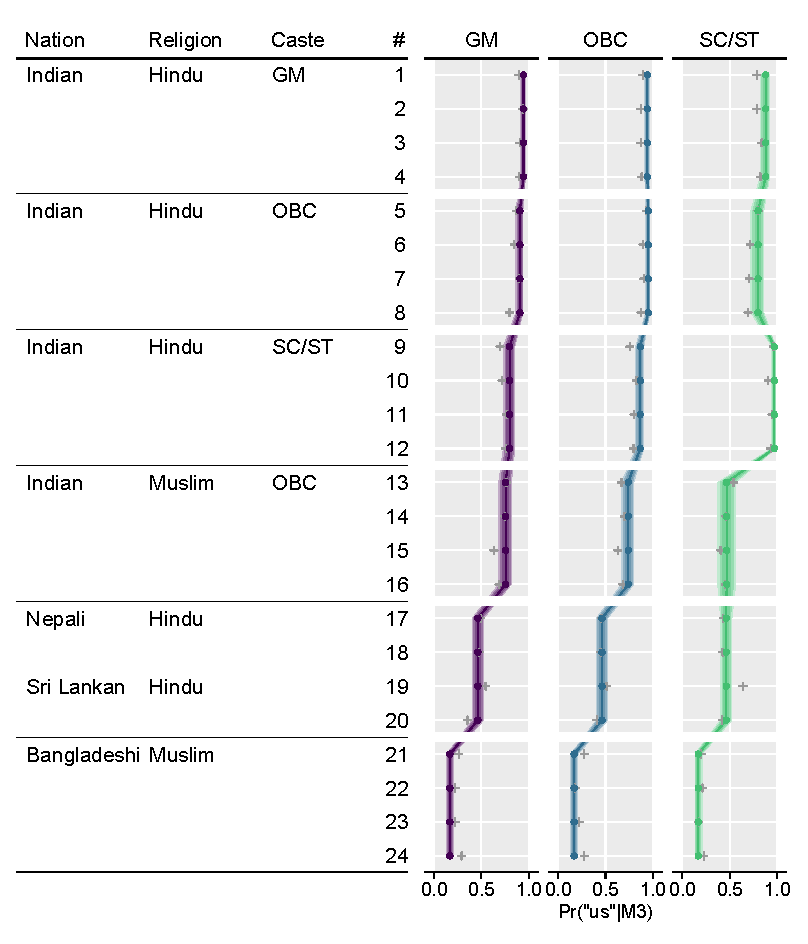
\includegraphics[scale=1]{../figures/figure-3}
\caption*{\textit{Note.} Dots (•) indicate the most plausible estimate for a given target’s probability of being included in participants’ ingroup, while the shaded ribbons encompass the 67\% (darkest shade), 89\%, and 97\% (lightest shade) most plausible estimates of that probability. Pluses (+) indicate the observed proportion of participants who included a given target in their ingroup. Comparing predicted and observed proportions shows that the model represents the data reasonably well. GM = General Merit, OBC = Other Backward Class, SC/ST = Scheduled Caste/Scheduled Tribe}
\label{fig:f3}
\end{figure}

As Figure~\ref{fig:f3} shows, we also found that how likely participants were to include Indian, Hindu targets in their ingroup varied as a function of both their own and the targets’ group membership. As predicted, GM participants (the most advantaged group) included Hindu, GM targets in their ingroup much more often than they included Hindu, SC/ST targets (the most disadvantaged group): $\Pr = .94, [.92, .97]$ versus $\Pr  = .80, [.73, .85]$, $\Delta\Pr = .14, [.09, .21]$. Likewise, SC/ST participants included Hindu, GM targets much less often than they included Hindu, SC/ST targets: $\Pr = .88, [.82, .92]$ versus $\Pr = .97, [.95, .98]$, $\Delta\Pr = -.09, [-.05, -.14]$. Both GM and SC/ST participants included targets from their own caste group more often than Hindu, OBC targets (the intermediate group): $\Delta\Pr = .04, [.08, >.00]$ and $\Delta\Pr = .17, [.24, .11]$, respectively. As hypothesized, we thus found strong evidence that participants from advantaged caste groups espoused social identities that excluded disadvantaged caste groups and vice versa.

Although we did not make clear predictions, we examined whether participants from the intermediate (OBC) group would espouse social identities that included targets from the advantaged (GM) group or the disadvantaged (SC/ST) group. Other than SC/ST participants, OBC participants included Hindu, GM targets in their ingroup as often as targets from their own caste group:  $\Pr = .94, [.92, .96]$ versus $\Pr = .95, [.93, .97]$, $\Delta\Pr = -.01, [-.04, .02]$. Like GM participants, OBC participants included targets from their own caste group more often than they included SC/ST targets:  $\Pr = .95, [.93, .97]$ versus $\Pr = .87, [.82, .90]$, $\Delta\Pr = .08, [.05, .13]$. This shows that participants from the intermediate group espoused social identities that included the most advantaged group, but not the most disadvantaged group.

\subsection{Individual differences}

Models 0--3 showed that group memberships shaped whom participants considered “us” and “not us”, though none of these associations were without exception. Models 4--7 examined to what extent individual differences in past experiences and ideological orientations explain why some participants excluded targets from caste and religious outgroups---and why others did not.

First, we compared Models 4--6 which tested whether intergroup contact was associated with how participants categorized Indians from caste and religious outgroups. Model 4 extended Model 3 by including contact quantity, positive contact, negative contact, and outgroup friendship as predictors of participants’ categorizations. As Table~\ref{tab:t2} shows, Model 4 made more accurate predictions than Model 3. Negative contact ($e^\beta = 0.81, [0.72, 0.91]$) and outgroup friendship ($e^\beta = 1.48, [1.28, 1.72]$) were associated with participants’ categorizations, but neither positive contact ($e^\beta = 1.01, [0.87, 1.16]$) nor contact quantity ($e^\beta = 0.99, [0.86, 1.14]$) were.\footnote{An odds ratio of $e^\beta = 1$ means that a predictor does not affect the odds of the relevant outcome; odds ratios of $e^\beta > 1$ and $e^\beta < 1$ mean, respectively, that a predictor makes the relevant outcome more and less likely.} Model 5 included only negative contact and outgroup friendship, and made more accurate predictions than Models 3 and 4. Model 6 extended Model 5 by estimating the relationships between contact and categorizations as varying across the four combinations of target caste and religion. Comparing the models’ Pseudo-BMA weights, we found that Models 5 ($w = .59$) and 6 ($w = .33$) both contributed to predicting participants’ categorizations. As Model 6, however, made somewhat less accurate predictions ($\Delta\textit{ELPD}/\textit{SE} = -0.5$), we selected the more parsimonious Model 5. We thus concluded that outgroup friendship and negative contact---but not contact quantity and positive contact---were associated with whom participants considered “us” and “not us”.

Second, we inspected estimates from Model 5 to examine whether the estimated coefficients were in the hypothesized direction. Figure~\ref{fig:f4} shows the estimated probabilities of participants categorizing targets as “us” as a function of their contact experiences. Across targets and participants, the odds of categorizing an outgroup target as “us” were $e^\beta = 1.48, [1.32, 1.68]$ times higher for each additional standard deviation of outgroup friendship. These odds were $e^\beta = 0.81, [0.72, 0.90]$ times lower for each standard deviation of negative contact. This means, for example, that GM participants who reported “never” having any negative contact with Muslims were more likely to categorize Indian Muslims as “us” than GM participants who reported “sometimes” having negative contact, $\Delta\Pr = .05, [.09, .03]$. GM participants who reported no friendships with Muslims were a lot less likely to include Indian Muslims in their ingroup than GM participants who had 2--5 Muslim friends with whom they “sometimes” spent time, $\Delta\Pr = .18, [.12, .24]$. 

\begin{figure}
\caption{Estimated probability of participants categorizing a target as “us” versus “not us” as a function of the targets’ group memberships (horizontal), the participants’ group memberships (colour), and the reported amount of negative contact and outgroup friendship with the relevant groups}
\centering
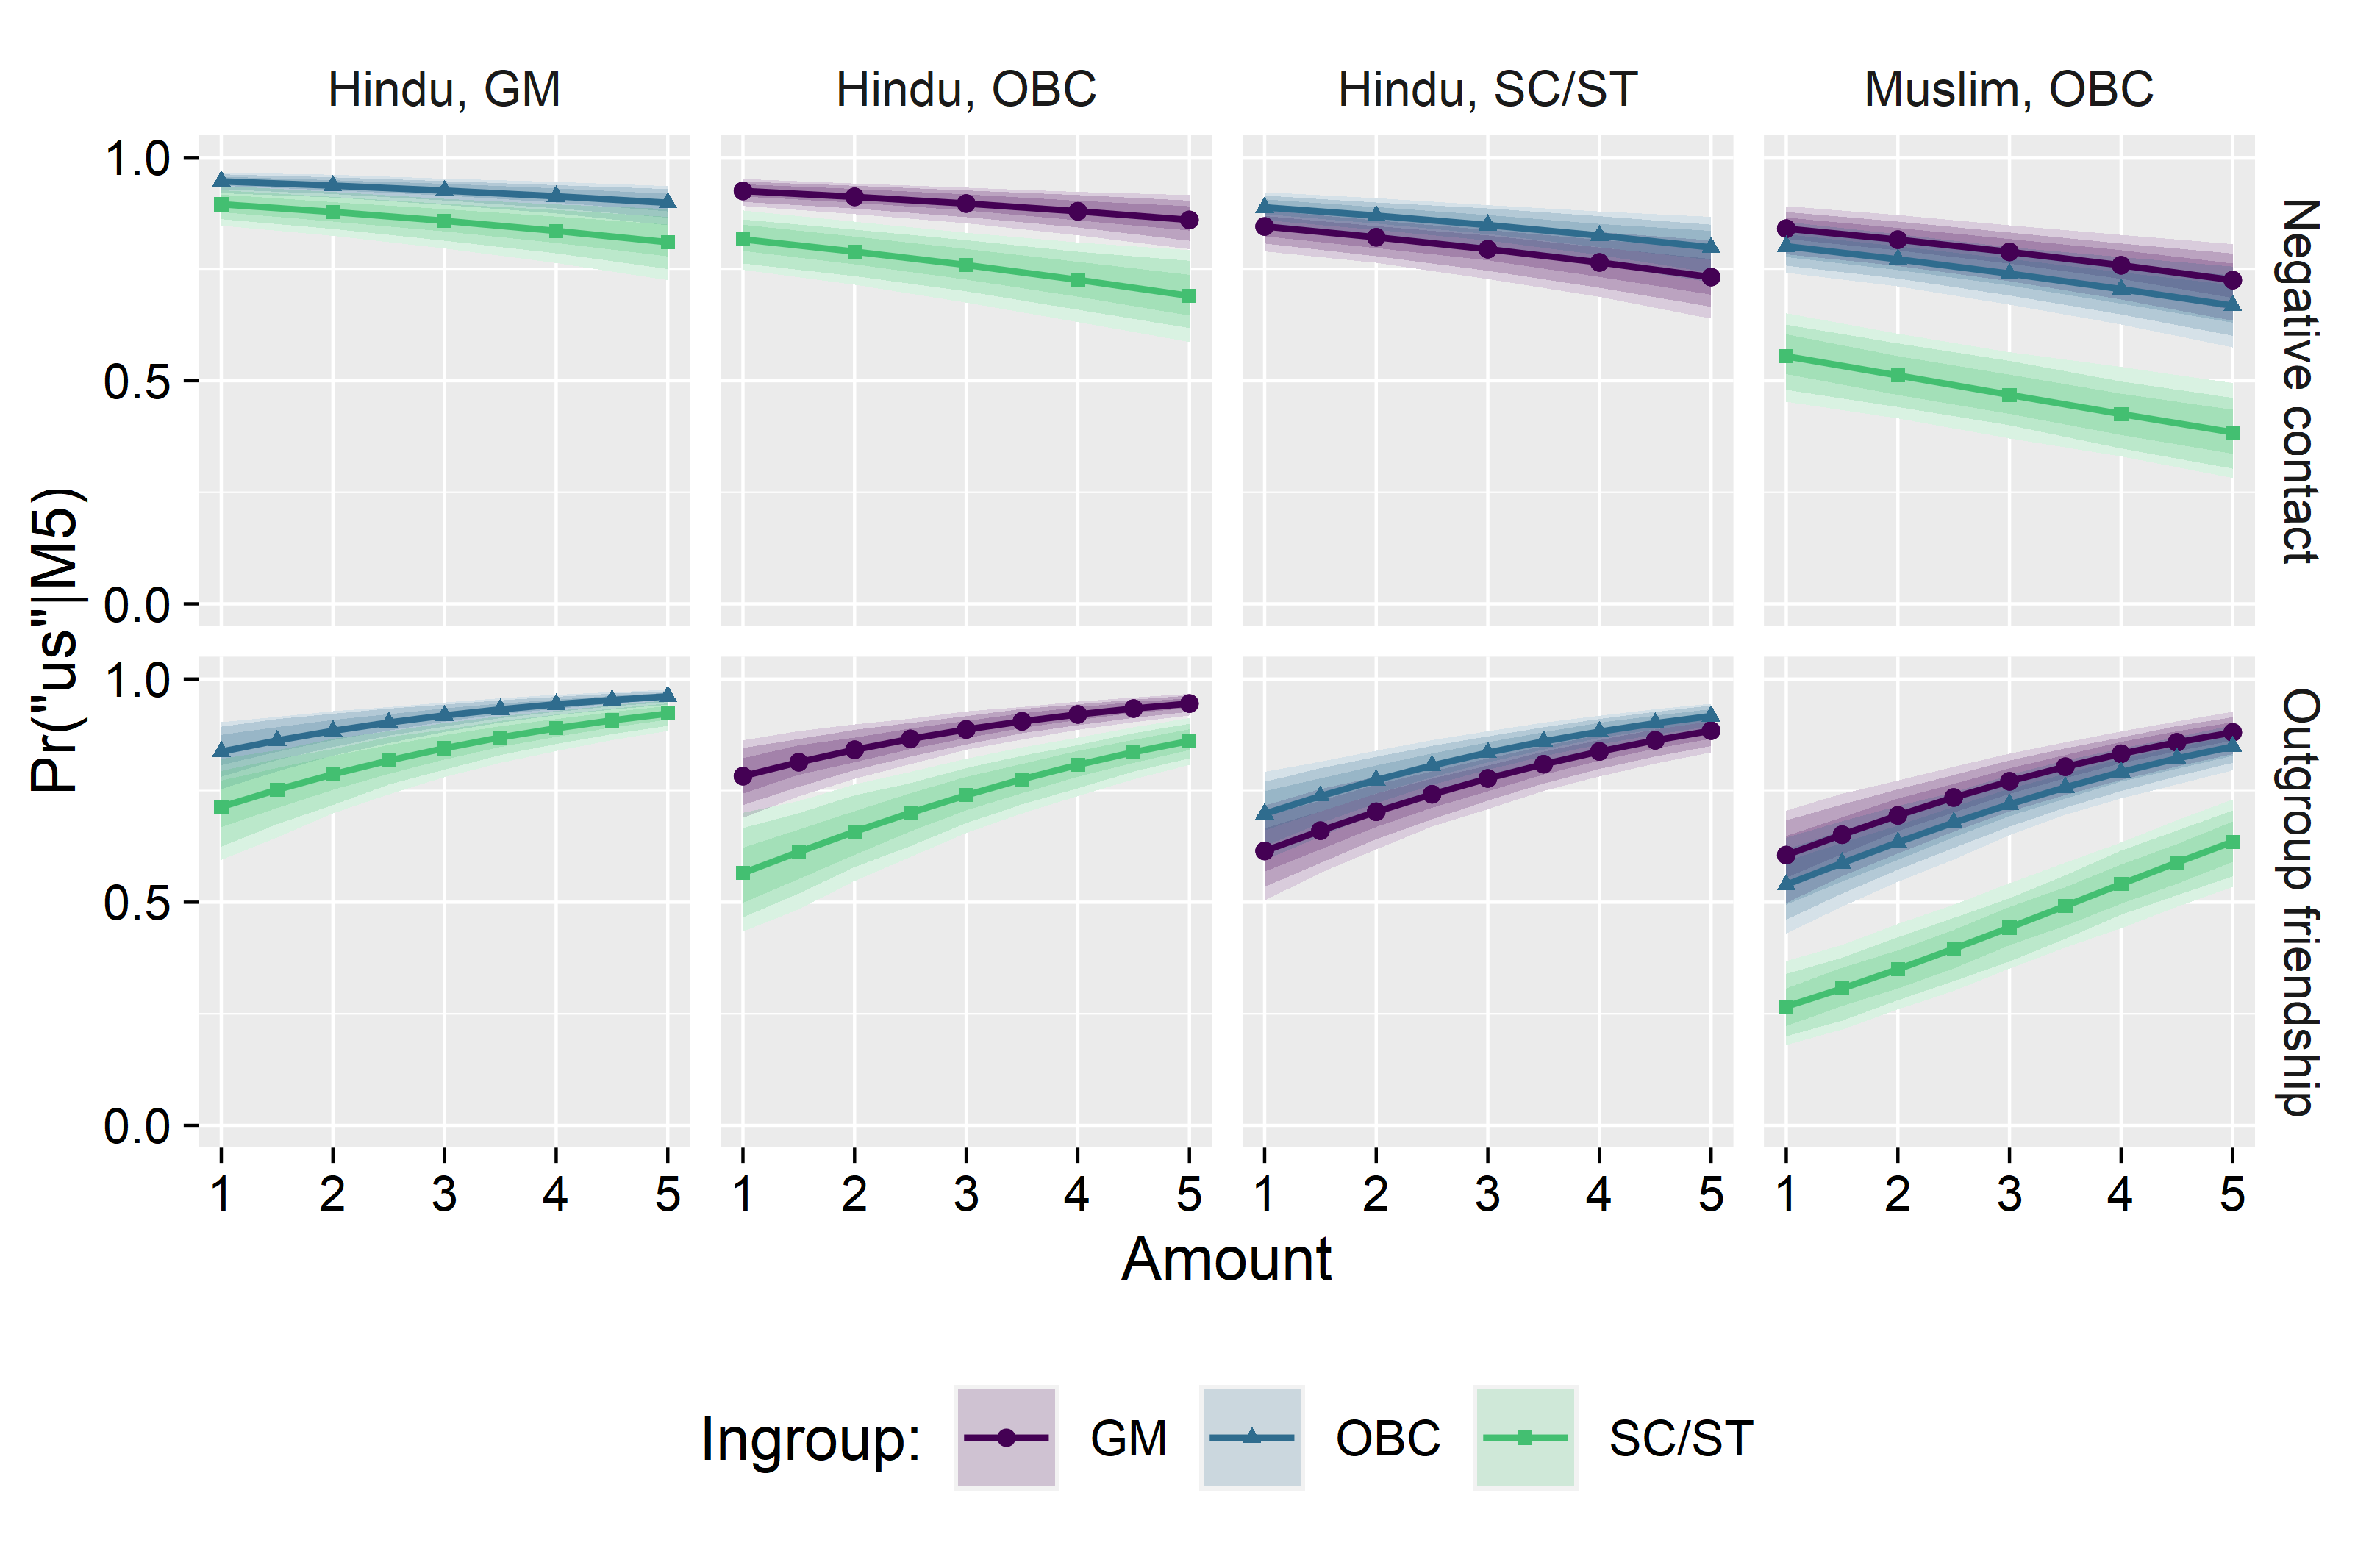
\includegraphics[scale=1]{../figures/figure-4}
\caption*{\textit{Note.} GM = General Merit, OBC = Other Backward Class, SC/ST = Scheduled Caste/Scheduled Tribe}
\label{fig:f4}
\end{figure}

Model 7 extended Model 3 by exploring whether social dominance orientation was associated with participants’ categorizations of targets from lower-status outgroups. Model 7 found little evidence for associations between participants’ categorizations and their SDO-Dominance scores ($e^\beta = 0.87, [0.69, 1.09]$) or SDO-Egalitarianism scores ($e^\beta = 0.99, [0.79, 1.24]$). Together, these findings show that group and individual differences explained whom participants included in their ingroup. As expected, past experiences with outgroup members explained why some participants included targets of (objective) caste or religions outgroups in their (subjective) ingroup, when others did not. In contrast, ideological orientations did not motivate participants to exclude lower-status groups.

\subsection{Consequences}

After examining potential antecedents, we turned to potential consequences of inclusive social identities. We analysed how participants’ categorizations related to their intergroup attitudes, their support for social change, and their perceptions of intergroup threat.

\subsubsection{Intergroup attitudes}

Across eight models, we examined how participants’ target-wise social distance and feeling thermometer ratings varied as a function of the targets’ and participants’ group memberships and of participants’ categorization. 

Models 0--3 estimated ratings (on either outcome) as varying across participants but fixed across targets (M0), as varying across target categories and participants (M1), and tested whether SC/ST participants’ responses differed from GM and OBC participants’ (M2), and whether OBC participants’ responses differed from GM participants’ (M3). As Table~\ref{tab:t3} shows, Models 1--3 improved upon the predictions of simpler models, showing that participants’ ratings depended on the targets’ and the participants’ group memberships.

\begin{table}
\caption{Comparison of multivariate linear regression models estimating participants’ social distance (SD) and feeling thermometer (FT) ratings as a function of group differences and target categorizations}
\centering
\figureversion{lining, tabular}
\small
\begin{tabularx}{\linewidth}{rXr@{~}rrr@{~}r@{~}r@{~}r} \toprule
\multicolumn{1}{c}{\textbf{(A)}} & \textit{\textbf{Group differences}} & \multicolumn{2}{c}{$R^2$} & \multicolumn{1}{l}{} & \multicolumn{4}{c}{$\Delta\textit{ELPD}/\textit{SE}$}                                                                                    \\ \cmidrule{6-9}
\#                               & Description                         & SD             & FT             & \textit{w}           & M0                          & M1                           & M2                           & M3                           \\ \midrule
M0                               & Varying intercept (Participants)    & .26            & .28            & .00                  & {\color[HTML]{E0E0E0} 0.0}  & {\color[HTML]{B2182B} -22.4} & {\color[HTML]{B2182B} -23.3} & {\color[HTML]{B2182B} -23.5} \\
M1                               & M0 + Varying intercept (Categories  & .39            & .44            & .00                  & {\color[HTML]{2166AC} 22.4} & {\color[HTML]{E0E0E0} 0.0}   & {\color[HTML]{B2182B} -5.7}  & {\color[HTML]{B2182B} -6.4}  \\
M2                               & M1 + Varying effect (SC/ST)         & .39            & .44            & .00                  & {\color[HTML]{2166AC} 23.3} & {\color[HTML]{2166AC} 5.7}   & {\color[HTML]{E0E0E0} 0.0}   & {\color[HTML]{D6604D} -3.1}  \\
M3                               & M2 + Varying effect (OBC)           & .40            & .45            & \textgreater .99     & {\color[HTML]{2166AC} 23.5} & {\color[HTML]{2166AC} 6.4}   & {\color[HTML]{4393C3} 3.1}   & {\color[HTML]{E0E0E0} 0.0}   \\ \bottomrule \addlinespace \toprule
\multicolumn{1}{c}{\textbf{(B)}} & \textit{\textbf{Consequences}}      & \multicolumn{2}{c}{$R^2$} & \multicolumn{1}{l}{} & \multicolumn{4}{c}{$\Delta\textit{ELPD}/\textit{SE}$}                                                                                    \\ \cmidrule{6-9}
\#                               & Description                         & SD             & FT             & \textit{w}           & M3                          & M4                           & M5                           & M6                           \\ \midrule
M3                               & Group differences (SC/ST, OBC)      & .40            & .45            & .00                  & {\color[HTML]{E0E0E0} 0.0}  & {\color[HTML]{B2182B} -9.3}  & {\color[HTML]{B2182B} -9.5}  & {\color[HTML]{B2182B} -9.1}  \\
M4                               & M3 + Fixed effect (Categorization)  & .43            & .47            & .01                  & {\color[HTML]{2166AC} 9.3}  & {\color[HTML]{E0E0E0} 0.0}   & {\color[HTML]{D6604D} -2.6}  & {\color[HTML]{E0E0E0} -1.5}  \\
M5                               & M4 + Varying effect (Categories)    & .43            & .48            & .88                  & {\color[HTML]{2166AC} 9.5}  & {\color[HTML]{4393C3} 2.6}   & {\color[HTML]{E0E0E0} 0.0}   & {\color[HTML]{E0E0E0} 1.2}   \\
M6                               & M5 + Interaction (SC/ST, OBC)       & .43            & .48            & .11                  & {\color[HTML]{2166AC} 9.1}  & {\color[HTML]{E0E0E0} 1.5}   & {\color[HTML]{E0E0E0} -1.2}  & {\color[HTML]{E0E0E0} 0.0}  \\ \bottomrule \addlinespace
\end{tabularx}
\label{tab:t3}
\caption*{\textit{Note.} $w$ is the weight of each model based on its relative out-of-sample prediction accuracy. $\Delta\textit{ELPD}/\textit{SE}$ is the difference in out-of-sample prediction accuracy between each pair of models, divided by its standard error. For a conventional interpretation, consider the critical values to be $|\Delta\textit{ELPD}/\textit{SE}| > 1.96$ for $p < .05$, 2.58 for $p < .01$, and 3.29 for $p < .001$ in a two-sided null-hypothesis significance test.}
\end{table}

Models 4--6 tested whether participants who categorized a target as “us” rated that target more favourably than participants who categorized the same target as “not us”. Models estimated this difference as constant across target categories (M4), as varying across target categories (M5), and tested whether this difference depended on participants’ caste memberships (M6). Models 4 and 5, but not Model 6, made better predictions than less complex models, showing that how favourably participants felt toward a target depended on whether they had categorized that target as “us” or “not us”, and that the size of this difference depended on the targets’---but not the participants’---group memberships.

Figure~\ref{fig:f5} shows the estimated social distance and feeling thermometer ratings as a function of target categorizations and participants’ group memberships. For all categories, participants felt more comfortable sharing a room with targets whom they categorized as “us” than with targets they categorized as “not us”. This difference was smallest for Indian, Hindu, GM targets ($\beta = 0.69, [0.33, 1.03]$; Cohen’s $d = 0.30, [0.14, 0.44]$) and greatest for foreign, Hindu targets ($\beta = 1.39, [1.14, 1.64]$; Cohen’s $d = 0.60, [0.49, 0.71]$). We found a similar pattern for feeling thermometer ratings. The difference was smallest for Indian, Hindu, OBC targets ($\beta = 8.3, [3.9, 12.7]$, Cohen’s $d = 0.25, [0.12, 0.39]$) and greatest for foreign, Hindu targets ($\beta = 21.1, [17.9, 24.4]$, Cohen’s $d = 0.64, [0.54, 0.74]$). Feeling thermometer and social distance ratings were highly correlated ($r = .58, [.56, .60]$). Categorizing a target as “us” was thus associated with more warmth and less social distance toward that target.

\begin{figure}
\caption{Posterior probabilities of social distance (\textbf{A}) and feeling thermometer (\textbf{B}) ratings as a function of target categorizations}
\centering
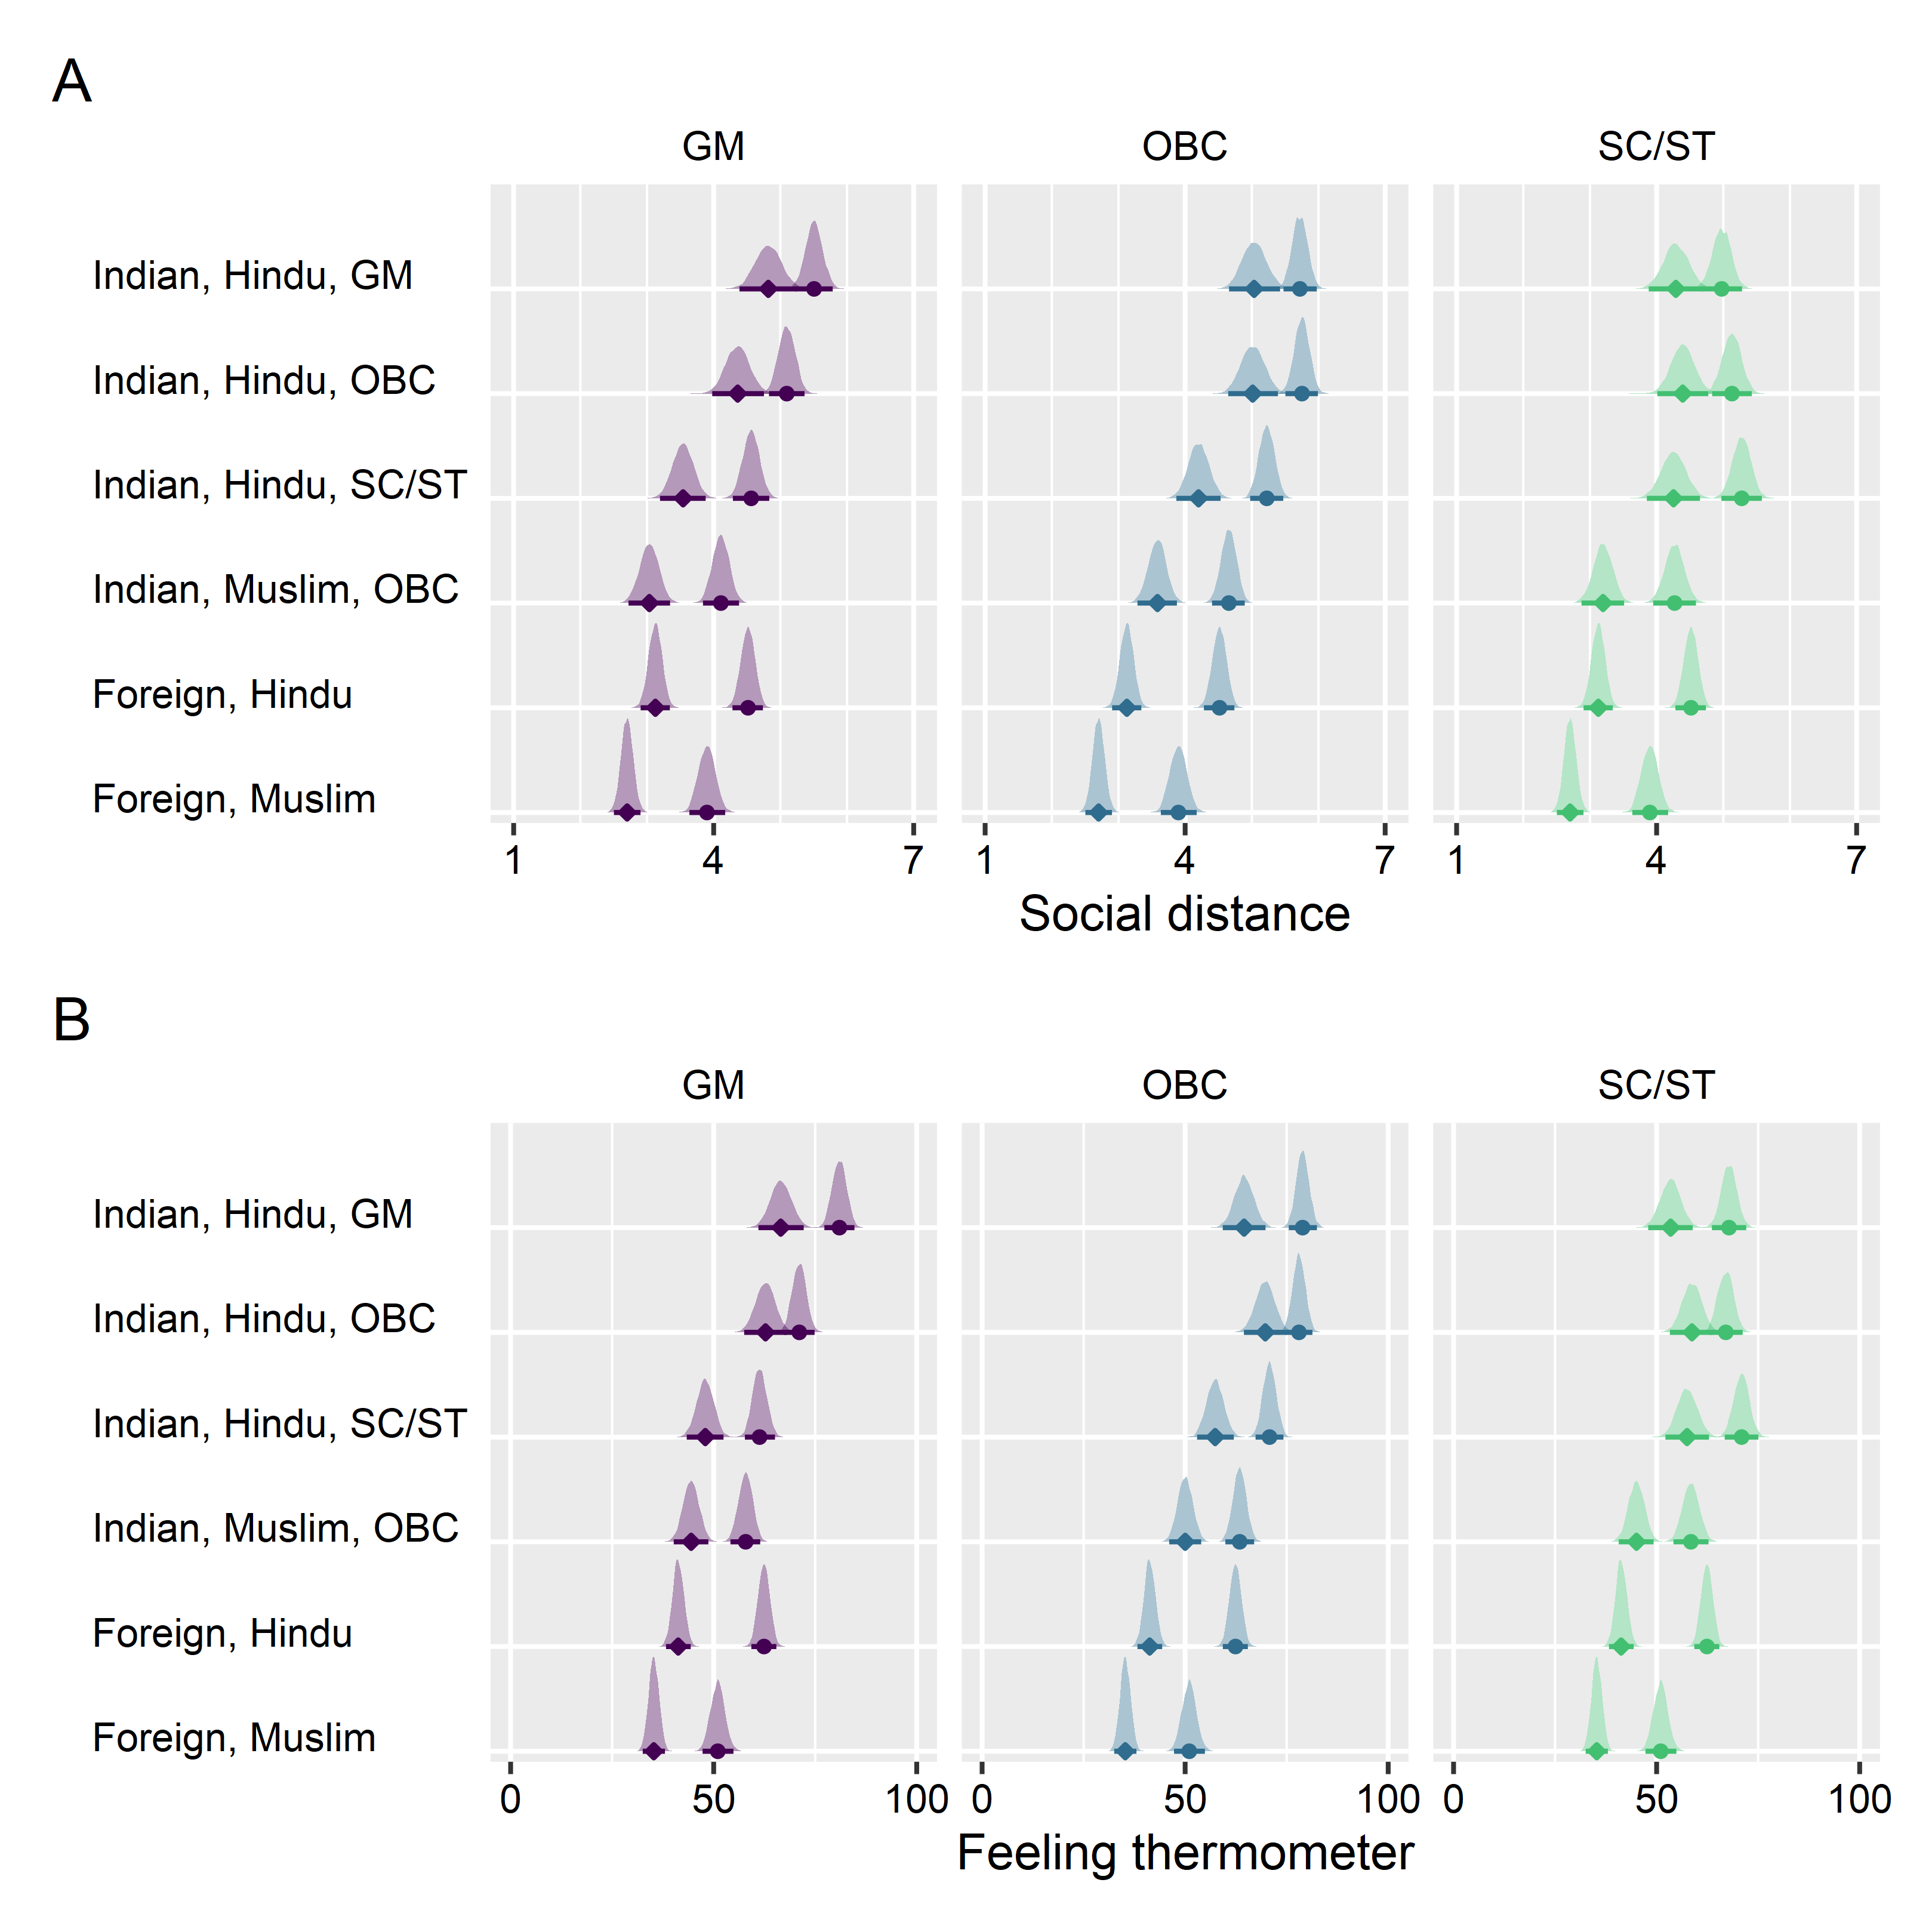
\includegraphics[scale=1]{../figures/figure-5}
\caption*{\textit{Note.} Points and diamonds mark the estimated mean ratings for targets categorized as “us” and “not us”, respectively. GM = General Merit, OBC = Other Backward Class, SC/ST = Scheduled Caste/Scheduled Tribe}
\label{fig:f5}
\end{figure}

\subsubsection{Support for social change}

Across four models, we examined how support for reservation policies benefiting SC/ST, OBC, and Muslim applicants varied as a function of the participants’ group memberships, their contact experiences, and their target categorizations. Model 0 estimated distinct means for the three target categories (SC/ST, OBC, Muslims). Model 1 extended Model 0 by estimating distinct means for GM, OBC, and SC/ST participants. As Table~\ref{tab:t4} shows, Model 1 made more accurate predictions than Model 0, showing that participants’ group memberships shaped their policy support ratings. 

\begin{table}
\caption{Comparison of multivariate linear regression models estimating participants’ policy support and perceived (dis-)advantage ratings as a function of group differences, intergroup contact, and target categorizations}
\centering
\figureversion{lining, tabular}
\small
\begin{tabularx}{\linewidth}{rXrrrrrr} \toprule
\textbf{(A)} & \textit{\textbf{Policy support}}            & \multicolumn{1}{l}{} & \multicolumn{1}{l}{} & \multicolumn{4}{c}{$\Delta\textit{ELPD}/\textit{SE}$}                                                                                \\ \cmidrule{5-8}
\#           & Description                                 & $R^2$          & \textit{w}           & M0                         & M1                          & M2                          & M3                          \\ \midrule
M0           & Group differences (Categories)              & .00                  & .00                  & {\color[HTML]{E0E0E0} 0.0} & {\color[HTML]{B2182B} -6.8} & {\color[HTML]{B2182B} -6.2} & {\color[HTML]{B2182B} -6.7} \\
M1           & M0 + Fixed effects (SC/ST + OBC)            & .22                  & .60                  & {\color[HTML]{2166AC} 6.8} & {\color[HTML]{E0E0E0} 0.0}  & {\color[HTML]{F4A582} 2.4}  & {\color[HTML]{E0E0E0} 0.3}  \\
M2           & M1 + Fixed effects (NC + OF)                & .24                  & .01                  & {\color[HTML]{2166AC} 6.2} & {\color[HTML]{92C5DE} -2.4} & {\color[HTML]{E0E0E0} 0.0}  & {\color[HTML]{FDDBC7} -1.7} \\
M3           & M1 + Fixed effects (Categorization)         & .23                  & .39                  & {\color[HTML]{2166AC} 6.7} & {\color[HTML]{E0E0E0} -0.3} & {\color[HTML]{D1E5F0} 1.7}  & {\color[HTML]{E0E0E0} 0.0}  \\ \bottomrule \addlinespace \toprule
\textbf{(B)} & \textit{\textbf{Perceived (dis-)advantage}} & \multicolumn{1}{l}{} & \multicolumn{1}{l}{} & \multicolumn{4}{c}{$\Delta\textit{ELPD}/\textit{SE}$}                                                                                \\ \cmidrule{5-8}
\#           & Description                                 & $R^2$ & \textit{w}           & M0                         & M1                          & M2                          & M3                          \\ \midrule
M0           & Group differences (Categories)              & .00                  & .04                  & {\color[HTML]{E0E0E0} 0.0} & {\color[HTML]{FDDBC7} -1.8} & {\color[HTML]{E0E0E0} -0.3} & {\color[HTML]{E0E0E0} -1.2} \\
M1           & M0 + Fixed effects (SC/ST + OBC)            & .04                  & .67                  & {\color[HTML]{D1E5F0} 1.8} & {\color[HTML]{E0E0E0} 0.0}  & {\color[HTML]{D1E5F0} 1.7}  & {\color[HTML]{E0E0E0} 0.7}  \\
M2           & M1 + Fixed effects (NC + OF)                & .06                  & .04                  & {\color[HTML]{E0E0E0} 0.3} & {\color[HTML]{FDDBC7} -1.7} & {\color[HTML]{E0E0E0} 0.0}  & {\color[HTML]{E0E0E0} -1.1} \\
M3           & M1 + Fixed effects (Categorization)         & .05                  & .25                  & {\color[HTML]{E0E0E0} 1.2} & {\color[HTML]{E0E0E0} -0.7} & {\color[HTML]{E0E0E0} 1.1}  & {\color[HTML]{E0E0E0} 0.0} \\ \bottomrule \addlinespace
\end{tabularx}
\label{tab:t4}
\caption*{\textit{Note.} $R^2$ is the mean $R^2$ across categories. $w$ is the weight of each model based on its relative out-of-sample prediction accuracy. $\Delta\textit{ELPD}/\textit{SE}$ is the difference in out-of-sample prediction accuracy between each pair of models, divided by its standard error. For a conventional interpretation, consider the critical values to be $|\Delta\textit{ELPD}/\textit{SE}| > 1.96$ for $p < .05$, 2.58 for $p < .01$, and 3.29 for $p < .001$ in a two-sided null-hypothesis significance test.}
\end{table}

Model 2 extended Model 1 by including outgroup friendship and negative contact as predictor variables: Model 2 estimated to what extent contact with the most advantaged (GM) caste group was associated with support for policies benefiting their own group among participants from the most disadvantaged (SC/ST) and intermediate (OBC) caste groups. Model 2 also estimated to what extent contact with SC/ST, OBC, and Muslim people was associated with support for policies benefitting these groups among participants not from these groups. As Model 2 made less accurate predictions than Model 3, we found no evidence that intergroup contact decreases policy support among the disadvantaged or increases policy support among the advantaged.

Model 3 extended Model 1 by including participants’ aggregated target categorizations as predictor variables: Model 3 tested whether the proportion of GM targets that SC/ST and OBC participants had considered “us” was associated with their support for policies benefiting their own group. Model 3 also tested whether the proportions of SC/ST, OBC and Muslim targets that participants had considered “us” was associated with support for policies benefitting these groups among participants not from these groups. Models 1 ($w = .60$) and 3 ($w = .39$) both contributed to predicting participants’ policy support ratings. As Model 3, however, made somewhat less accurate predictions ($\Delta\textit{ELPD}/\textit{SE} = -0.4$), we selected the more parsimonious Model 1. We thus concluded that participants’ policy support ratings depended on their own group memberships, but not on their contact experiences and target categorizations.

\begin{figure}
\caption{Posterior probabilities of policy support ratings for different target groups (right) by participants’ caste ingroup (left)}
\centering
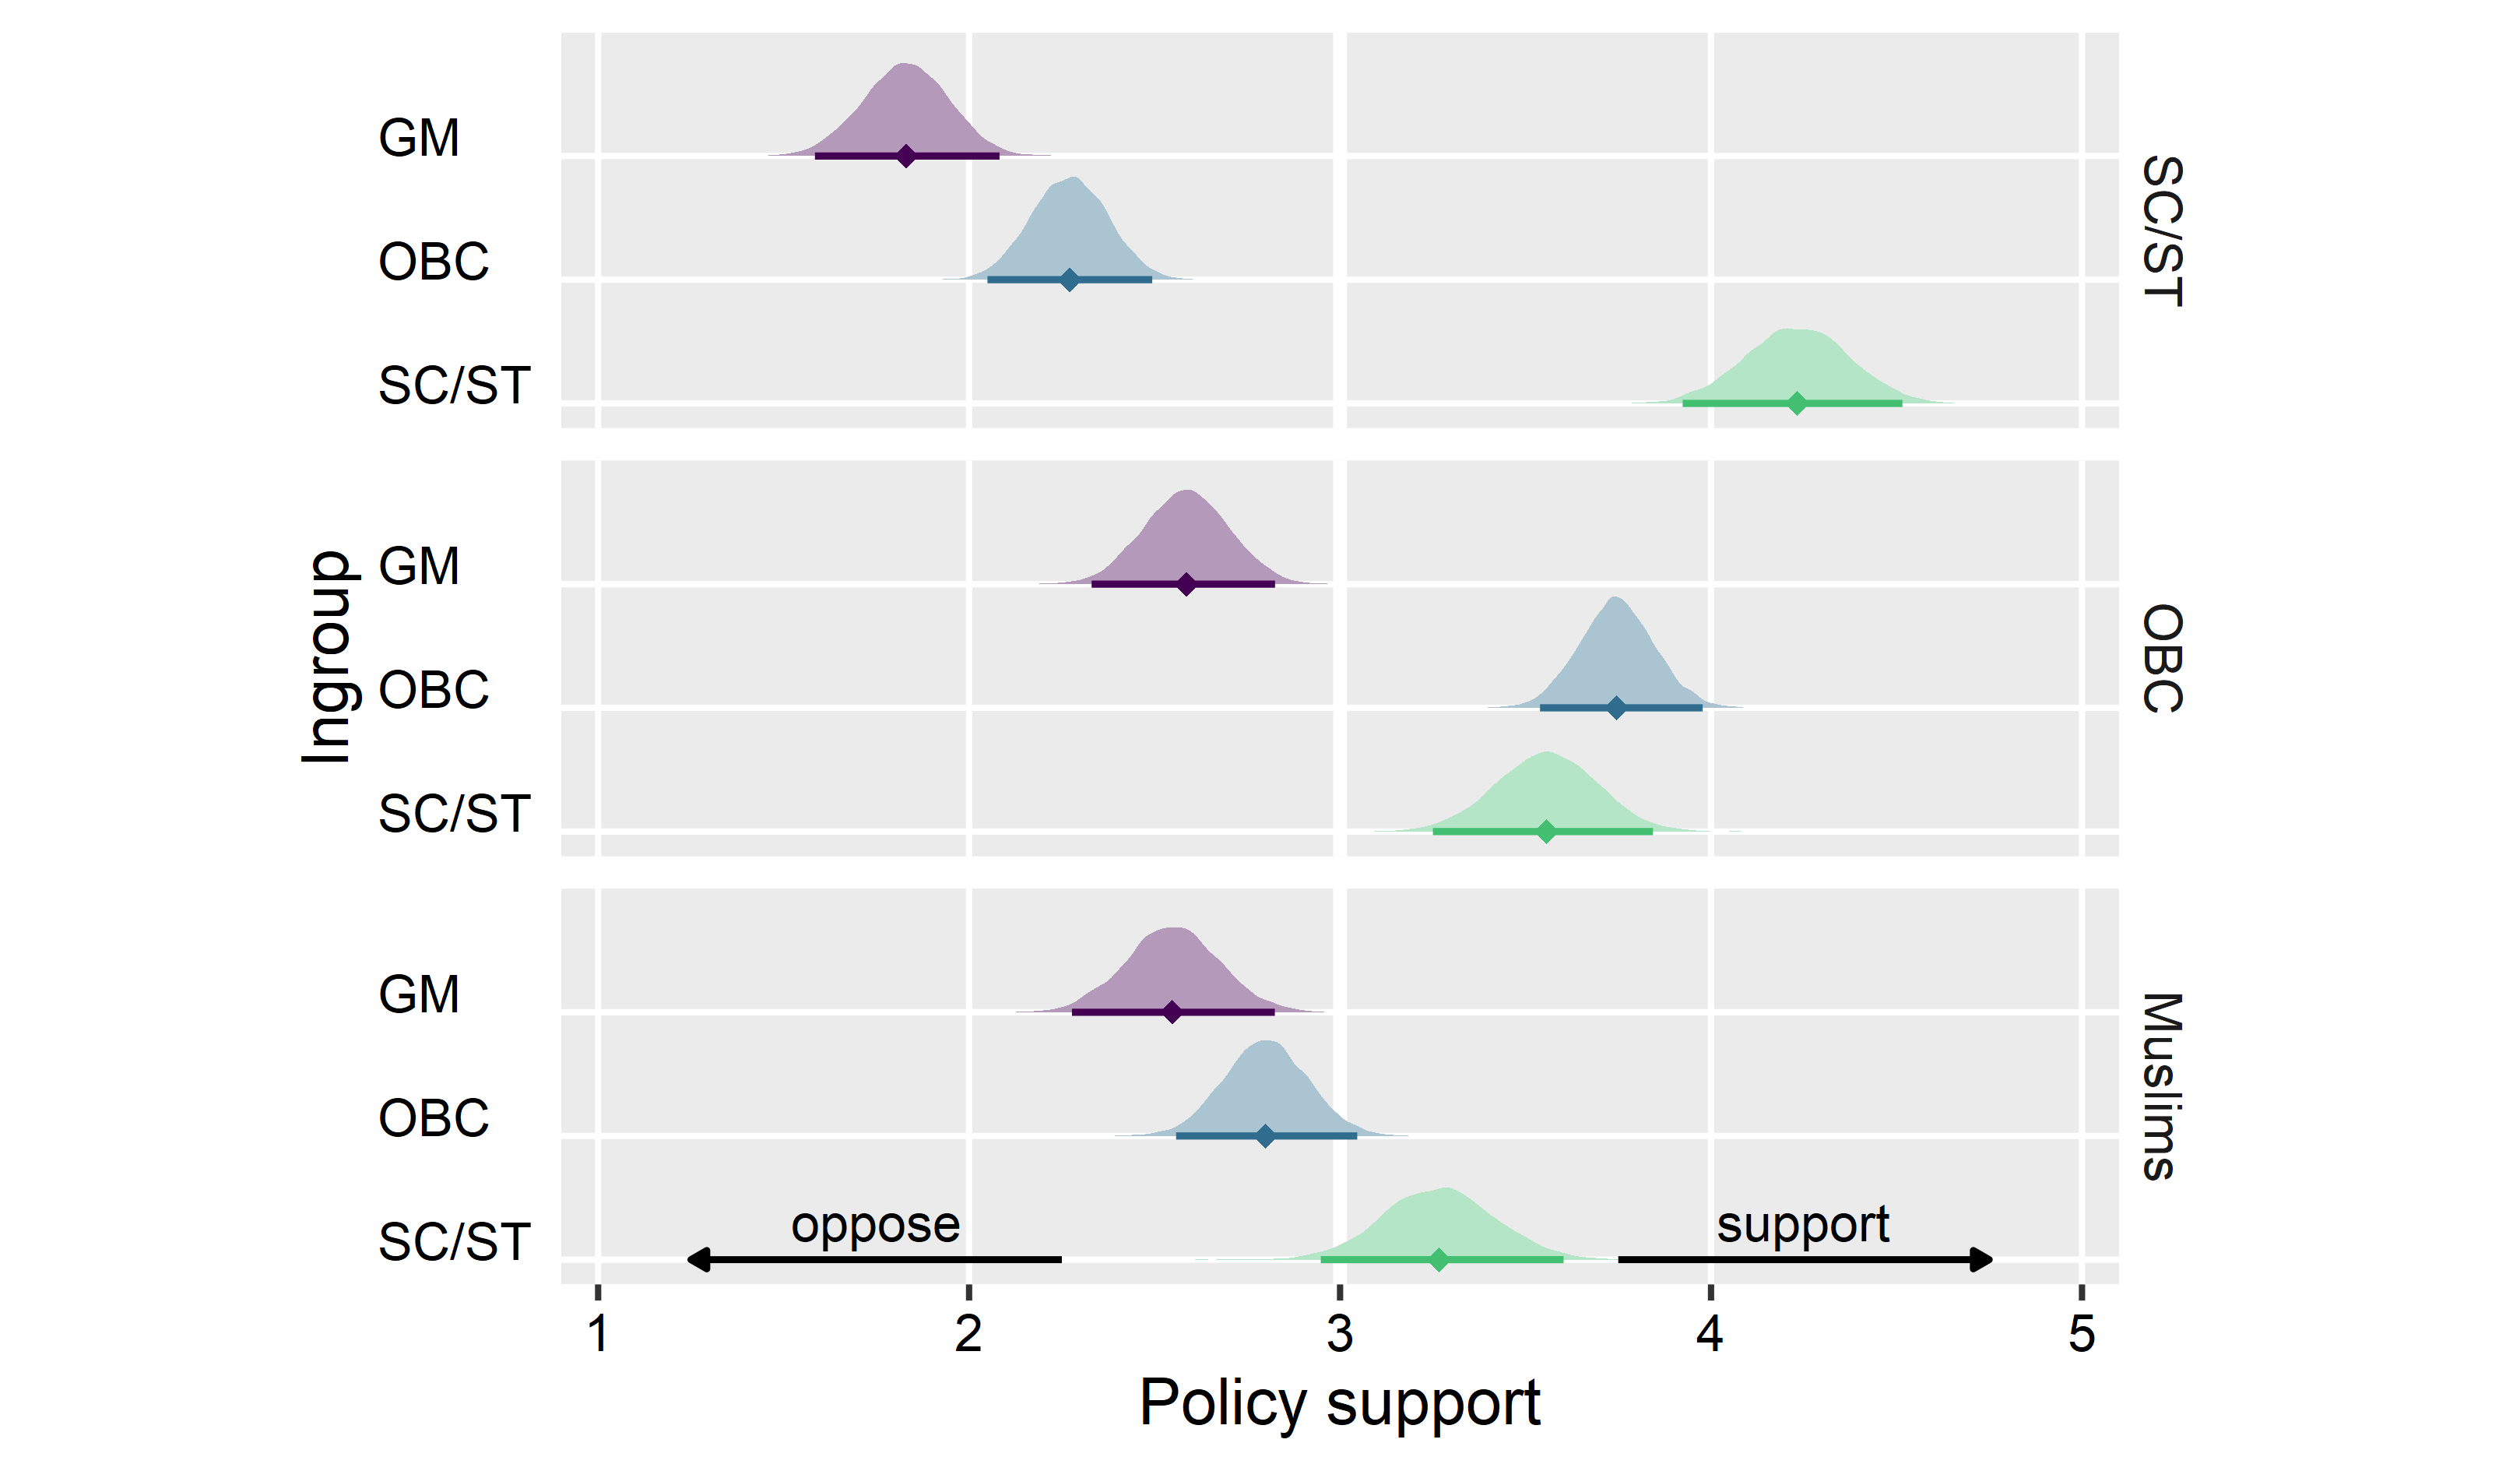
\includegraphics[scale=1]{../figures/figure-6}
\caption*{\textit{Note.} Diamonds are the point estimates of each mean rating while intervals encompass the 97\% most plausible estimates. GM = General Merit, OBC = Other Backward Class, SC/ST = Scheduled Caste/Scheduled Tribe.}
\label{fig:f6}
\end{figure}

\begin{figure}
\caption{Posterior probabilities of perceived (dis-)advantage ratings for different target groups (right) by participants’ caste ingroup (left)}
\centering
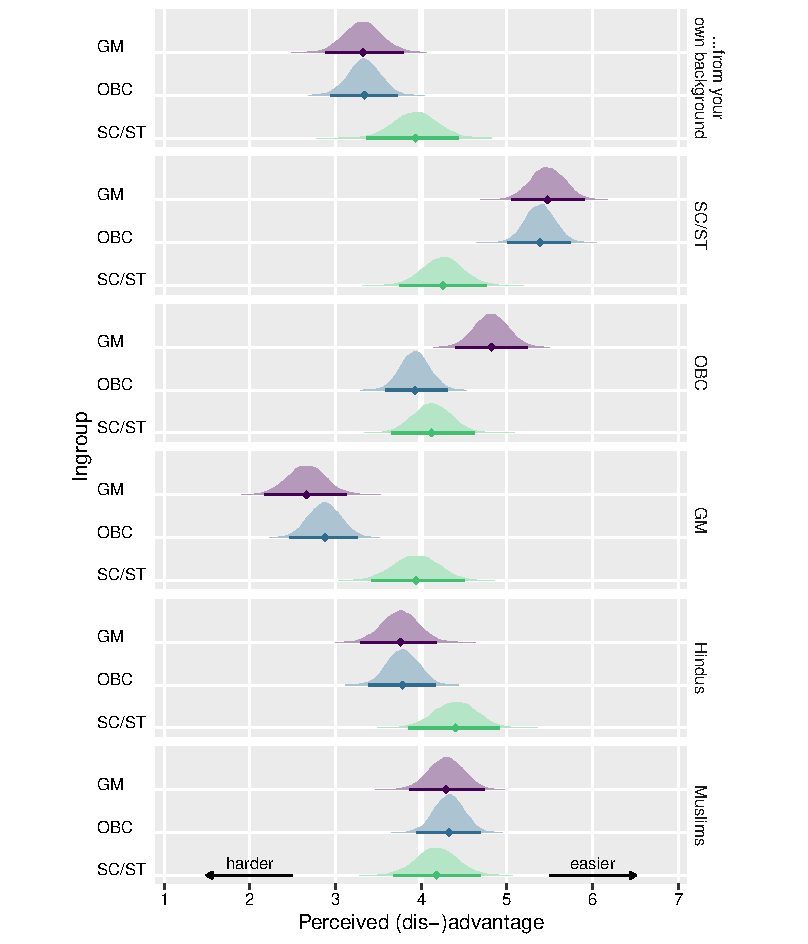
\includegraphics[scale=1]{../figures/figure-7}
\caption*{\textit{Note.} Diamonds are the point estimates of each mean rating while intervals encompass the 97\% most plausible estimates. GM = General Merit, OBC = Other Backward Class, SC/ST = Scheduled Caste/Scheduled Tribe.}
\label{fig:f7}
\end{figure}


Figure 6 shows the estimated group differences in policy support ratings. We found that policy support was strongly aligned with participants’ caste interests. SC/ST participants supported reservations for both SC/ST and OBC students, while OBC participants only supported reservations for their own group. GM participants, for the most part, opposed reservation policies. We estimated a similar set of four models with participants’ perceived (dis-)advantage ratings as outcome variables. As Table~\ref{tab:t4} shows, we again found Model 1 to make the most accurate out-of-sample predictions. Figure  7 shows the estimated group differences in perceived (dis-)advantage ratings. We found that, contradicting prevailing social inequalities, GM and OBC participants rated their own groups’ lives as substantially harder than SC/ST members’ lives. Contrary to our predictions, we did not find more inclusive identities or intergroup contact to be associated with perceived (dis-)advantage or policy support ratings.

\subsubsection{Intergroup threat}

We also explored to what extent participants’ perceptions of realistic and symbolic threat depended on how inclusive their identity construals were. Results from a series of multilevel models showed that participants reported more realistic ($M = 3.62, [3.49, 3.75]$) than symbolic ($M = 3.21, [3.09, 3.33]$) threat from (same-religion) Dalits, but more symbolic ($M = 3.47, [3.34, 3.61]$) than realistic ($M = 3.23, [3.06, 3.38]$) threat from (different-religion) Muslims. Contrary to predictions, we did not find that participants felt less threatened by Muslims and Dalits if they categorized more targets from these outgroups as “us” (for details, see Appendix E).

Overall, we thus found that when participants included a person in their ingroup, they had, on average, more favourable attitudes to and desired less social distance from that person. Participants’ categorizations, however, were unrelated to perceptions of intergroup threat and relative (dis-)advantage and to support for affirmative action.

\section{Discussion}

We examined how people construct their social identities from multiple social categories and how more inclusive identities relate to intergroup contact, outgroup attitudes, and support for social change. As hypothesized, we found that cross-group friendship was associated with more inclusive identities which, in turn, were associated with more favourable outgroup attitudes. Negative contact was associated with less inclusive identities. Contrary to past research, neither intergroup contact nor more inclusive identities were associated with perceived (dis-)advantages or support for affirmative action. Below, we discuss implications, strengths, and limitations of this research.

\subsection{Implications}

Our research has implications for understanding intergroup relations in unequal societies. Among advantaged groups, our research documented patterns of inclusion/exclusion that map onto persistent social divides. Participants from dominant caste groups tended to exclude subordinate caste groups from the common ingroup; participants from the dominant Hindu religion tended to exclude Indian Muslims. Among disadvantaged groups, we found more complex patterns. Participants from intermediate caste groups (OBC, Other Backward Classes) faced the choice of aligning themselves with dominant caste groups (GM, General Merit) or forming a coalition with subordinate caste groups (SC/ST, Scheduled Caste/Scheduled Tribe). OBC participants tended to include dominant GM targets and exclude subordinate SC/ST targets, thus choosing derogation over coalition \parencite{craig_coalition_2012}. Similarly, SC/ST participants rejected a solidarity-based social identity that includes Indian Muslims.

Our findings suggest that cross-group friendship can help to overcome these divisions by fostering social identities that include Indians of all castes and religions. As more inclusive identities were related to less social distance and more warmth toward caste and religious minorities, our research suggests that positive contact could help reduce interpersonal discrimination and violence against these groups. In line with recent research \parencite{hayward_toward_2017}, we found that negative contact could exacerbate social divisions by fostering less inclusive identities. More broadly, our research speaks to \emph{how} contact reduces prejudice \parencite{pettigrew_how_2008}. Our findings support arguments \parencite{gaertner_reducing_2000, pettigrew_intergroup_1998} that contact can reduce prejudice, in part, by changing how we understand our social identities.

Our research also examined support for social change. Contrary to past research, neither positive nor negative contact \parencite{hayward_how_2018, reimer_intergroup_2017} were associated with support for social change---or perceptions of relative advantage and disadvantage---in advantaged \parencite{selvanathan_whites_2018, dixon_intergroup_2007} and disadvantaged \parencite{dixon_beyond_2012} groups. Similarly, more inclusive identities were not associated with opposition to affirmative action among the disadvantaged \parencite{dixon_attitudes_2012}. Features of the participants’ situation might explain this discrepancy. As university students, participants have personally experienced the impact of reservation policies. For SC/ST and OBC students, reservation policies facilitated admission to state-funded universities. This experience might explain why these students strongly support reservation (at least for their own group). For GM students, reservation policies thwarted admission to state-funded universities. This experience might explain why, in contrast to societal realities, GM students saw themselves at a disadvantage relative to other caste groups \parencite[see][]{norton_whites_2011}.

Our research has practical implications for intergroup relations in today’s India. On the one hand, our findings help explain recent developments in Hindu---Muslim relations. Since we conducted this study, the Hindu-nationalist BJP government was re-elected and enacted the Citizenship Amendment Act which excluded Muslims from a newly-opened path to Indian citizenship \parencite{noauthor_citizenship_2019}. Many Indians, including Hindus, protested the bill and for a more inclusive nationalism. These protests, in turn, were met with violent backlash, fomented by BJP politicians, culminating in an anti-Muslim pogrom in Delhi \parencite{kamdar_what_2020}. In line with our findings, these developments highlight the deleterious consequences of exclusive social identities. On the other hand, our findings point to cross-group friendship as a means to foster inclusive social identities. Reservation policies, which reserve seats for caste and (in some states) religious minorities, make universities promising avenues for intergroup contact. Just as our findings revealed strong opposition to reservation policies by advantaged caste groups, our findings thus also provide evidence of the importance of reservation policies for facilitating intergroup contact.\footnote{This is not to suggest that these instrumental benefits matter more than their role in addressing past and current injustices.}

\subsection{Strengths and limitations}

Our findings show that the triple crossed-categorization task \parencite{van_dommelen_construing_2015} is an intuitive and informative method for studying social identification across multiple categories. We adapted the task to answer new questions about social identification. First, we recruited respondents from multiple groups, allowing us to study both individual and group differences \parencite[see also][]{brankovic_social_2016}. Second, we estimated responses as varying across targets and participants using multilevel models. This allowed more fine-grained analyses than the quantitative and qualitative summaries provided by van Dommelen and colleagues, and may explain why we found more consistent effects of intergroup contact. Together, these changes open the task to a broader range of research questions.

Our research also improves upon other approaches to studying identification across multiple social categories. For example, we could have tested our hypotheses by examining whether intergroup contact leads participants to identify with a more inclusive common ingroup (Indians) instead of their less inclusive subordinate ingroups (Hindus). A problem with this approach is that people tend to perceive the common ingroup as more similar to their own narrow ingroup than to subordinate outgroups \parencite{wenzel_ingroup_2003}, thus excluding outgroup members from the common ingroup. Instead, we allowed participants to decide where to draw the line between ingroup and outgroup and to thus determine the content of their subjective ingroup. Another strength of our research is that we studied intergroup relations in a context underrepresented in psychological research. Our research is one of few studies examining the effects of intergroup contact on Hindu–Muslim relations in South Asia \parencite[for other examples, see][]{islam_dimensions_1993, tausch_relationships_2009} and is, to our knowledge, the first study examining the effects of intergroup contact on caste relations.

Despite these strengths, our research is qualified by some methodological limitations. We presented all participants with the same combination of target groups. This within-subjects design cannot determine whether the observed construals generalize beyond the specific combination of stimuli used. For example, participants might have relied on the specific combination of stimuli to rank target groups and to decide where to draw the line between “us” and “not us”---suggesting that we would find smaller group differences in a between-subjects design. Another limitation is that the within-subjects design limited the number of categories we could consider without overburdening participants. Class, rather than caste, could explain why some participants excluded targets from disadvantaged outgroups. Gender could have intersectional effects on whom participants consider “us” and “not us”---for example, by activating different stereotypes about Muslim men and Muslim women. Future research should combine the advantages of within- and between-subjects designs by using a planned missingness design in which each participant views a sample of stimuli from a larger set that includes more combinations of categories than is feasible in a within-subjects design.

Another limitation is that we measured categorization and attitudes for the same targets. This design cannot rule out that these variables measure the same construct, rather than represent a genuine association across constructs. One reason to think so is that intergroup threat, a more distal measure, did not correlate with participants’ categorizations.\footnote{An explanation might be that threat perceptions stem from economic anxieties (e.g., fearing affirmative action as a threat to one’s career) and ideological beliefs (e.g., Hindutva), rather than identity processes.} A final limitation is we did not manipulate intergroup contact. This design cannot rule out confounding explanations of the observed relationship between contact and identification. Experimental studies tend to manipulate short-term ‘intergroup interactions’ rather than long-term ‘intergroup contact’ (MacInnis \& Page-Gould, \cite*{macinnis_how_2015}; for rare exceptions, see Laar et al., \cite*{laar_effect_2005}, and Shook \& Fazio, \cite*{shook_interracial_2008}). Our findings suggest, however, that cross-group friendship, not superficial interaction, is required for people to change their social identities. Future research should address these limitations by assessing intergroup bias with proximal and distal measures and by testing the hypothesized relationships over time.

\section{Conclusion}

To conclude, in a unique study of caste, religion, and nationality in South India, we found correlational evidence that intergroup contact can change not only how we see others, but also how we see ourselves---that is, that intergroup contact can foster more inclusive social identities and thus improve intergroup relations in unequal societies. Fostering more inclusive identities, however, does not seem to overcome entrenched opposition to (or undermine support for) affirmative action.

\newpage

\printbibliography

\end{document}
